\documentclass[12pt]{article}
\usepackage[margin=1in]{geometry}
\usepackage[portuges,english]{babel} % Portuguese language support (English is the main language)
%\usepackage[a4paper,margin=1in,footskip=0.20in]{geometry}
\newcommand{\ignore}[1]{}
\geometry{left=1in,right=1in,top=0.95in,bottom=1in}

%%%%%%%%%%%%%%%%%%%%%%%%%%%%%%%%%%%%%%%%%%%%%%%%%%%%%%%%%%%%%%%%%%%%%%%%%%%%%%%%%%%%%%%%%%%%%%%%%%%%%%%%%%%%%%%%%%%%%%%%%%%%%%%%%%%%%%%%%%%%%%%%%%%%%%%%%%%%%%%%%%%%%%%%%%%%%%%%%%%%%%%%%%%%%%%%%%%%%%%%%%%%%%%%%%%%%%%%%%%%%%%%%%%%%%%%%%%%%%%%%%%%%%%%%%%%

\usepackage[title]{appendix}
\usepackage{changepage}
\usepackage{subcaption}
\usepackage{csquotes}
\usepackage{adjustbox}
\usepackage[graphicx]{realboxes}
\usepackage{longtable}
\usepackage[utf8]{inputenc}
\usepackage{titleps}
\usepackage[affil-it]{authblk}
%\usepackage[margin=1in]{geometry}
\usepackage{setspace}
\usepackage{sectsty}
\usepackage{titling}
\usepackage{titletoc}
\usepackage{pifont}
\usepackage{ragged2e}
\usepackage{fancyhdr}
%\usepackage{subfig}
%\usepackage{graphicx}
% Tables and Figures
\usepackage{lscape}
\captionsetup{labelfont={bf,sf},justification=centering,font=small}
\usepackage{float}
\usepackage{indentfirst}
\usepackage{rotating}
\usepackage{multicol}
\usepackage{multirow}
\usepackage{booktabs}
\usepackage{lipsum}
\usepackage{tikz}
\usetikzlibrary{decorations.pathreplacing, positioning, arrows.meta}
\definecolor{myLightGray}{RGB}{191,191,191}
\definecolor{myGray}{RGB}{160,160,160}
\definecolor{myDarkGray}{RGB}{144,144,144}
\definecolor{myDarkRed}{RGB}{167,114,115}
\definecolor{myRed}{RGB}{255,58,70}
\definecolor{myGreen}{RGB}{0,255,71}
\usepackage{colortbl}

\interfootnotelinepenalty=-200 %% Completely prevent breaking of 
\usepackage[para,online,flushleft]{threeparttable}


\usepackage{newfloat}
\DeclareFloatingEnvironment[
name=Figure,
within=section,
]{suppfigure}
\DeclareFloatingEnvironment[
name=Table,
within=section,
]{supptable}


%\usepackage{bigfoot}
%\global\dimen\footins = 4cm

%\usepackage[nofiglist,notablist,tabhead,fighead]{endfloat}


% Citations
\usepackage{natbib}
\newcommand{\citetapos}[1]{\citeauthor{#1}'s \citeyearpar{#1}}

% References in Appendix
\usepackage{multibib}
\newcites{sec}{References}

% Math environment
\usepackage{amsfonts}
\usepackage{amsmath}
\usepackage{amssymb}
\usepackage{amsthm}
\usepackage{commath}
\usepackage{bbm}
\usepackage[nottoc]{tocbibind}

\usepackage{nicefrac}
\newcommand{\xmark}{\ding{55}}%

\newtheorem{theorem}{Theorem}
\newtheorem{assumption}{Assumption}
\newtheorem{definition}{Definition}
\newtheorem{lemma}{Lemma}[]
\newtheorem{proposition}[theorem]{Proposition}
\newtheorem{propapen}{Proposition}[section]
\renewcommand{\qedsymbol}{\ensuremath{\blacksquare}}

\renewcommand{\vec}[1]{\mathbf{#1}}



\sectionfont{\large}
\subsectionfont{\normalsize\mdseries\itshape}

% Invisible section
\newcommand\invisiblesection[1]{%
  \refstepcounter{section}%
  \addcontentsline{toc}{section}{\protect\numberline{\thesection}#1}%
  \sectionmark{#1}}

% Space within tabular
\renewcommand{\arraystretch}{1.2}

\newpagestyle{online}{%
  \sethead{}{}{\bf For Online Publication}%
  \setfoot{}{\thepage}{}%
  \setheadrule{0pt}%
  \setfootrule{0pt}%
}

\renewcommand{\thesubsubsection}{\thesubsection.\Alph{subsubsection}}

% https://tex.stackexchange.com/questions/291603/how-to-put-hyperlinks-in-endfloats-markers
%\usepackage[nolists]{endfloat}
%\usepackage{mwe}
%\usepackage{subcaption}


%\renewcommand{\footnotesize}{\fontsize{12pt}{13pt}\selectfont}

\usepackage[pdfborder={0 0 0 [0 0]}, colorlinks=FALSE, urlcolor=magenta,	 citecolor=red, filecolor=magenta, bookmarks=TRUE, pdftitle={Subways and Local Income Growth: Evidence from Brasília},	 pdfauthor={Lucas Dutra}]{hyperref}

\hypersetup{
    colorlinks = {true},
    citecolor={blue},
    urlcolor={blue},
    linkcolor = {blue}
    }

\usepackage{xr-hyper}
\makeatletter
\newcommand*{\addFileDependency}[1]{% argument=file name and extension
  \typeout{(#1)}
  \@addtofilelist{#1}
  \IfFileExists{#1}{}{\typeout{No file #1.}}
}
\makeatother
 
\newcommand*{\myexternaldocument}[1]{%
    \externaldocument{#1}%
    \addFileDependency{#1.tex}%
    \addFileDependency{#1.aux}%
}
\myexternaldocument{Paper_appendix}



\newgeometry{top=1in,bottom=1in,right=1in,left=1in}

\makeatletter
\providecommand{\floatplace}[1]{}%
\renewcommand{\floatplace}[1]{% #1 = float type (e.g. figure)
   \begin{center}
     \def\floatnumber{\csname thepost#1\endcsname}
     \def\floatname{\csname #1name\endcsname}
     \hypertarget{figureback\floatnumber}{}%
     \@ifundefined{#1anchor\floatnumber}%
       {[\floatname~\floatnumber\ about here.]}%
       {\hyperlink{\csname #1anchor\floatnumber\endcsname}%
         {[\floatname~\floatnumber\ about here.]}}
   \end{center}}

\newcommand{\figurecaption}[2][\empty]% #1=short caption (optional), #2=caption
 {\ifx\empty#1\relax \caption[#2]{\hyperlink{figureback\thefigure}{#2}}%
  \else \caption[#1]{\hyperlink{figureback\thefigure}{#2}}%
  \fi
  \immediate\write\@auxout{\string\newfigure{\thefigure}{\@currentHref}}}
\makeatother

\newcommand{\newfigure}[2]% #1 = \thefigure, #2 = \@currentHref
  {\expandafter\gdef\csname figureanchor#1\endcsname{#2}}
 
\makeatletter
%for table
\newcommand{\tabcaption}[2][\empty]% #1=short caption (optional), #2=caption (tabcaption instead of tablecaption for glossaries)
{%
    \ifx\empty#1\relax %
        \caption[#2]{\hyperlink{tableback\thetable}{#2}}%
    \else %
        \caption[#1]{\hyperlink{tableback\thetable}{#2}}%
    \fi
    \immediate\write\@auxout{\string\newtable{\thetable}{\@currentHref}}%
}
\makeatother

\newcommand{\newtable}[2]% #1 = \thetable, #2 = \@currentHref
{\expandafter\gdef\csname tableanchor#1\endcsname{#2}}


% %########################## TITLE PAGE ########################### 


 \title{Subways and Local Income Growth: Evidence from Brasília}



\author{%
    \href{}{Lucas Dutra de Paulo}\thanks{Universidade Católica de Brasília, Brasil, e-mail:
    \href{mailto:lucasdutra0099@gmail.com}{lucasdutra0099@gmail.com}.} 
}




% %\affil{\small Catholic University of Brasília, Brazil}




 \providecommand{\keywords}[1]{\textbf{\textit{Keywords:}} #1}
 \providecommand{\jel}[2]{\textbf{\textit{JEL Codes:}} #1}

\date{\small \today}




 \begin{document}

\maketitle

\renewcommand{\abstractname}{Abstract}
% \selectlanguage{english}
\begin{abstract}


\noindent Evidence that mass transit raises local income does not settle whether the gains reach the residents who already lived in the areas it serves, and most of it comes from advanced economies. This paper addresses this gap by studying the effect of the Brasília subway on local income. Brasília, a planned capital whose core is legally protected from densification, is an extreme case of a city where residents cannot move closer to jobs. Using census-tract data for 2000 and 2010 and an instrumental-variable strategy based on a planned and discarded subway alignment, we find that tracts exposed to the subway experienced income growth approximately 10 percent higher than comparable unexposed tracts. We find no evidence that this gain reflects physical restructuring of exposed areas or the replacement of lower-income residents by wealthier ones. In addition, both the share of household heads with positive income and the average income of those who already had it rise more in exposed tracts, consistent with a labor-market channel. Overall, the results indicate that, where moving closer to jobs is not an option, a subway can raise the income of the residents who stay.

\noindent
\end{abstract}

\keywords{Mass transit; Income; Brasília.}\

\jel{O18, R11, R23, R42.}

% \doublespacing
% \thispagestyle{empty}
\clearpage

\onehalfspacing


\section{Introduction}\label{S:introduction}

Cities worldwide continue to invest heavily in urban rail systems to connect residents to job centers \citep{uitp2024globalmetro}, yet whether these investments raise the incomes of the residents they serve remains an open question. Much of the existing evidence speaks instead to capitalization into property values: transit access raises housing prices near stations and along transport corridors \citep{diaz1999impacts, cohen2007impacts, wrigley2001transport, koutsopoulos1977impact, hess2007impact}. Whether this value reaches residents as real income growth---rather than being captured by landowners or dissipated through residential turnover---is far less settled: the estimated effect of transit proximity on local income ranges from positive to null to negative, depending on selection into treated areas and on how commuting and displacement are measured \citep{banerjee2020road, fogel1962quantitative, fogel1964railroads}.

Most of the empirical evidence on this question comes from advanced economies \citep{mohammad2013meta, gonzalez2018subways}, while mass transit is plausibly more consequential for income in developing-country cities, where the evidence base is thinner and commuting costs and uneven transit provision loom larger \citep{tsivanidis2026evaluating, storeygard2025transportLMIC, moreno2016access, iimi2019jobaccessibility}. In this context of developing-country cities, this paper turns to Brasília, Brazil's capital. Brasília's modernist core and central business district (CBD), the \textit{Plano Piloto}, is a purpose-built urban design with rigid land-use rules and limited housing capacity: much of the city's growth has been absorbed by satellite cities farther from the center, even as employment and public services remain highly concentrated in the core \citep{de2025evolution, unesco1987brasilia, acioly1992brasilia}. Because the \textit{Plano Piloto} is legally protected from densification, Brasília blocks the channel that \cite{glaeser2018economic} show usually connects workers to a city's income gains: where housing supply can expand, residents move closer to jobs and share in the income gains of the productive core. Where densification is blocked, as in Brasília, that option disappears: residents cannot move closer to jobs, and any income gains are instead capitalized into housing prices rather than reaching residents directly. Mass transit is a substitute for this blocked channel: workers cannot move closer to the center, but the subway can shorten their commute to it, so income gains are more likely to reach current residents directly rather than being captured only by whoever can afford to move in. Brasília therefore represents an extreme version of a situation common to many cities with expensive, supply-constrained centers: when moving closer to jobs is not an option, can transit still raise the incomes of the workers who stay?

In this context, this paper investigates whether the construction and operation of the Brasília Subway System increased income growth in areas exposed to the system, and, in particular, whether that growth reflects real income gains among the residents who already lived there rather than a shift in who lives there. To do so, we use IBGE census-tract data for Brasília in 2000, before the subway was implemented, and 2010, when the subway was already in operation, and use income growth over the decade as the main outcome. To perform this analysis, we use an instrumental-variables approach that leverages a planned and discarded subway alignment to address the potential endogeneity of station placement, controlling for baseline tract characteristics and administrative-region fixed effects. First, we estimate whether census tracts exposed to the subway experienced higher income growth between 2000 and 2010 than non-exposed tracts. Second, we subject these estimates to a battery of robustness checks that vary the geographic scope of the comparison group, the distance threshold used to define treatment, and the functional form of the exposure measure, assessing whether the main finding holds across alternative specification choices. Third, and crucially for the interpretation of the first set of results, we ask whether that income growth represents real gains for the residents who already lived in exposed tracts, by testing three hypotheses. Two rule out alternative explanations: that the effect reflects changes in the physical structure of exposed areas, or demographic sorting, meaning higher-income households replace lower-income incumbents. The third hypothesis adds a direct, positive argument for the same conclusion. Since job access itself cannot be measured directly, the labor-market hypothesis asks whether household-head income moved the way improved job access would predict: a larger share of household heads earning some income, and existing earners earning more.

Our results indicate that census tracts exposed to a subway station experienced income growth approximately 10 percent higher than otherwise comparable tracts over the 2000–2010 decade, a positive and statistically significant effect that is consistent across specifications with increasingly comprehensive sets of controls. This estimate holds across different specification tests: the point estimate remains positive and of similar magnitude when the geographic scope of the comparison group is varied, when the distance threshold used to define treatment is varied, and when the binary exposure indicator is replaced by continuous intensity-based measures of proximity. To assess whether this result reflects real income gains among incumbent residents, three mechanisms are tested. Two are alternative explanations: an urban structure hypothesis, under which income growth follows from subway-induced physical densification rather than from improved labor-market access; and a demographic composition hypothesis, under which tract-level income rises through the displacement of lower-income residents and their replacement by wealthier ones. Neither finds support in the data. Having ruled out both, the third hypothesis supplies a direct, positive argument for the same conclusion. Because job access cannot be measured directly, the labor-market hypothesis is tested by decomposing the income effect into an extensive margin---the share of household heads with positive income---and an intensive margin---the average income of those who already had it. Both margins respond positively and significantly to subway exposure, evidence that the income effect reflects real income gains among the residents already living in subway-exposed areas, consistent with the labor-market channel.

This paper is related to a literature asking whether mass transit raises local income, and more specifically, whether it raises the income of the residents who already lived there. Transport investments are thought to reshape a city's economic geography by changing how its residents interact with it---cheaper, faster connections change where people can realistically work relative to where they live \citep{duranton2012urban}. For mass transit specifically, a few studies find that it raises local income. \citet{heilmann2018transit}, exploiting a Dallas rail network that was extensively planned but only partially built, finds that census tracts that received light-rail access saw their median family income rise relative to tracts that were promised access but did not receive it. \citet{yen2024rapid}, instrumenting station placement in Los Angeles with a hypothetical least-cost Metro route, finds that residents living near new stations saw their earnings rise by as much as 26 percent. \citet{mayertrevien2017largescale} find a comparable employment gain, 12.8 percent, in municipalities connected to a new commuter-rail line in the Paris region. What none of these studies can settle is whose income rose.

In each case, the authors themselves attribute part or all of the gain to a change in who lives or works in the area rather than to income growth among incumbent residents. \citet{heilmann2018transit} attributes Dallas's income gain to housing turnover: poorer households move out as land near stations grows more valuable, wealthier ones move in, and the tract's income rises without any resident's income doing so. \citet{mayertrevien2017largescale} report the same pattern for Paris: population overall is unaffected, but the share of high-skill residents rises near new stations, which they interpret as ``a population displacement effect: a shift toward more wealthy residents around new stations'' rather than income growth for anyone already there. \citet{tyndall2021local} finds the same pattern across four U.S. metros: light rail stations raise neighborhood-level employment, but a structural neighborhood-choice model shows this operates by pricing low-skilled workers out of accessible areas and into more isolated ones, so that light rail transit lowers aggregate metropolitan employment even as it raises it locally. \citet{yen2024rapid} reaches a related but distinct conclusion: earnings near new Los Angeles stations rise most where local job density also rises, suggesting the gain reflects new economic activity moving into the area rather than existing residents reaching jobs they could not reach before. A credible claim that a subway raised the incomes of its existing residents has to rule out both of these stories---compositional change and physical or economic restructuring of the area---not merely report a positive coefficient on tract income. This is a demanding standard, and one that developing-country cities have not yet been held to: the evidence above comes entirely from cities in the United States and France, while commuting costs and the returns to closing a job-access gap are plausibly larger where transit provision is thinner and more uneven \citep{tsivanidis2026evaluating}.

This paper is built to close that gap, contributing to the literature on mass transit and urban economic outcomes in three ways. First, it provides causal evidence on the income effects of subway exposure in a developing-country context, where commuting frictions, labor-market structure, and spatial inequality differ substantially from the settings that dominate the empirical literature, and where the welfare consequences of transit investment may therefore be qualitatively different. Second, the paper contributes methodologically by exploiting a planned and subsequently discarded subway alignment as an instrument for realized station proximity, and by conducting the analysis at the fine-grained census-tract level. Third, unlike \citet{heilmann2018transit}, \citet{mayertrevien2017largescale}, and \citet{tyndall2021local}, who attribute comparable local gains to a change in who lives or works in the exposed area, this paper shows that the income gains documented here are accompanied by neither: they reflect real income growth among the residents who already lived in exposed tracts, closing the gap left open above.

The present paper is structured as follows. Section~\ref{s:subway} describes the Brasília subway system, its history, spatial configuration, and the planned and discarded alignment used as the instrument. Section~\ref{s:data} describes the census-tract data, the construction of the exposure and instrument measures, and presents descriptive statistics. Section~\ref{s:methodology} presents the empirical strategy, detailing the 2SLS approach, the construction of the exposure and instrument variables, and the role of administrative-region fixed effects. Section~\ref{s:results} presents the main estimates and a series of robustness tests that vary the geographic scope of the comparison group, the distance threshold used to define treatment, and the functional form of the exposure measure. Section~\ref{s:mechanisms} investigates the mechanisms behind the estimated income effect, ruling out urban structure changes and demographic composition shifts in subway-exposed areas before testing the labor-market channel directly. Finally, Section~\ref{s:conclusion} presents the paper's conclusions.

\section{The Brasília Subway System}\label{s:subway}

Proposals for a rail-based transit system in the Federal District predate its construction by more than two decades. A preliminary plan was presented to the local government in 1976 but was judged unfeasible. A formal feasibility study was subsequently commissioned from the Mauá Institute of Technology (\textit{Instituto Mauá de Tecnologia}, IMT) in 1986--1987, which produced a network design that was set aside in favor of further studies; the project eventually built corresponded to a later design, contracted under a subsequent administration. Construction began in 1992 but was marked by repeated interruptions driven by hyperinflation and contested federal transfers. Commercial service started only in September 2001, more than seven years after the original target date, and the network was subsequently expanded over the following two decades.

In its current configuration, the system comprises two operating lines---the Green Line and the Orange Line---totaling 27 stations across 42 km of track \citep{institutomdt2019evolucao}. The two lines run from Central station, in the \textit{Plano Piloto}, and bifurcate toward Ceilândia and Samambaia via Taguatinga, serving six administrative regions in total. Because of the long distances between many stations and the low residential densities along the corridor, the system functions largely as an inter-regional connector rather than as a fine-grained intra-urban network. Figure~\ref{fig:subway_system} maps the network and names the six administrative regions it serves, making explicit the corridor running from Central station, in the \textit{Plano Piloto}, westward to Ceilândia and Samambaia.

\begin{figure}[h!]
\caption{The Brasília Subway System and the Administrative Regions It Serves}
\label{fig:subway_system}
\centering
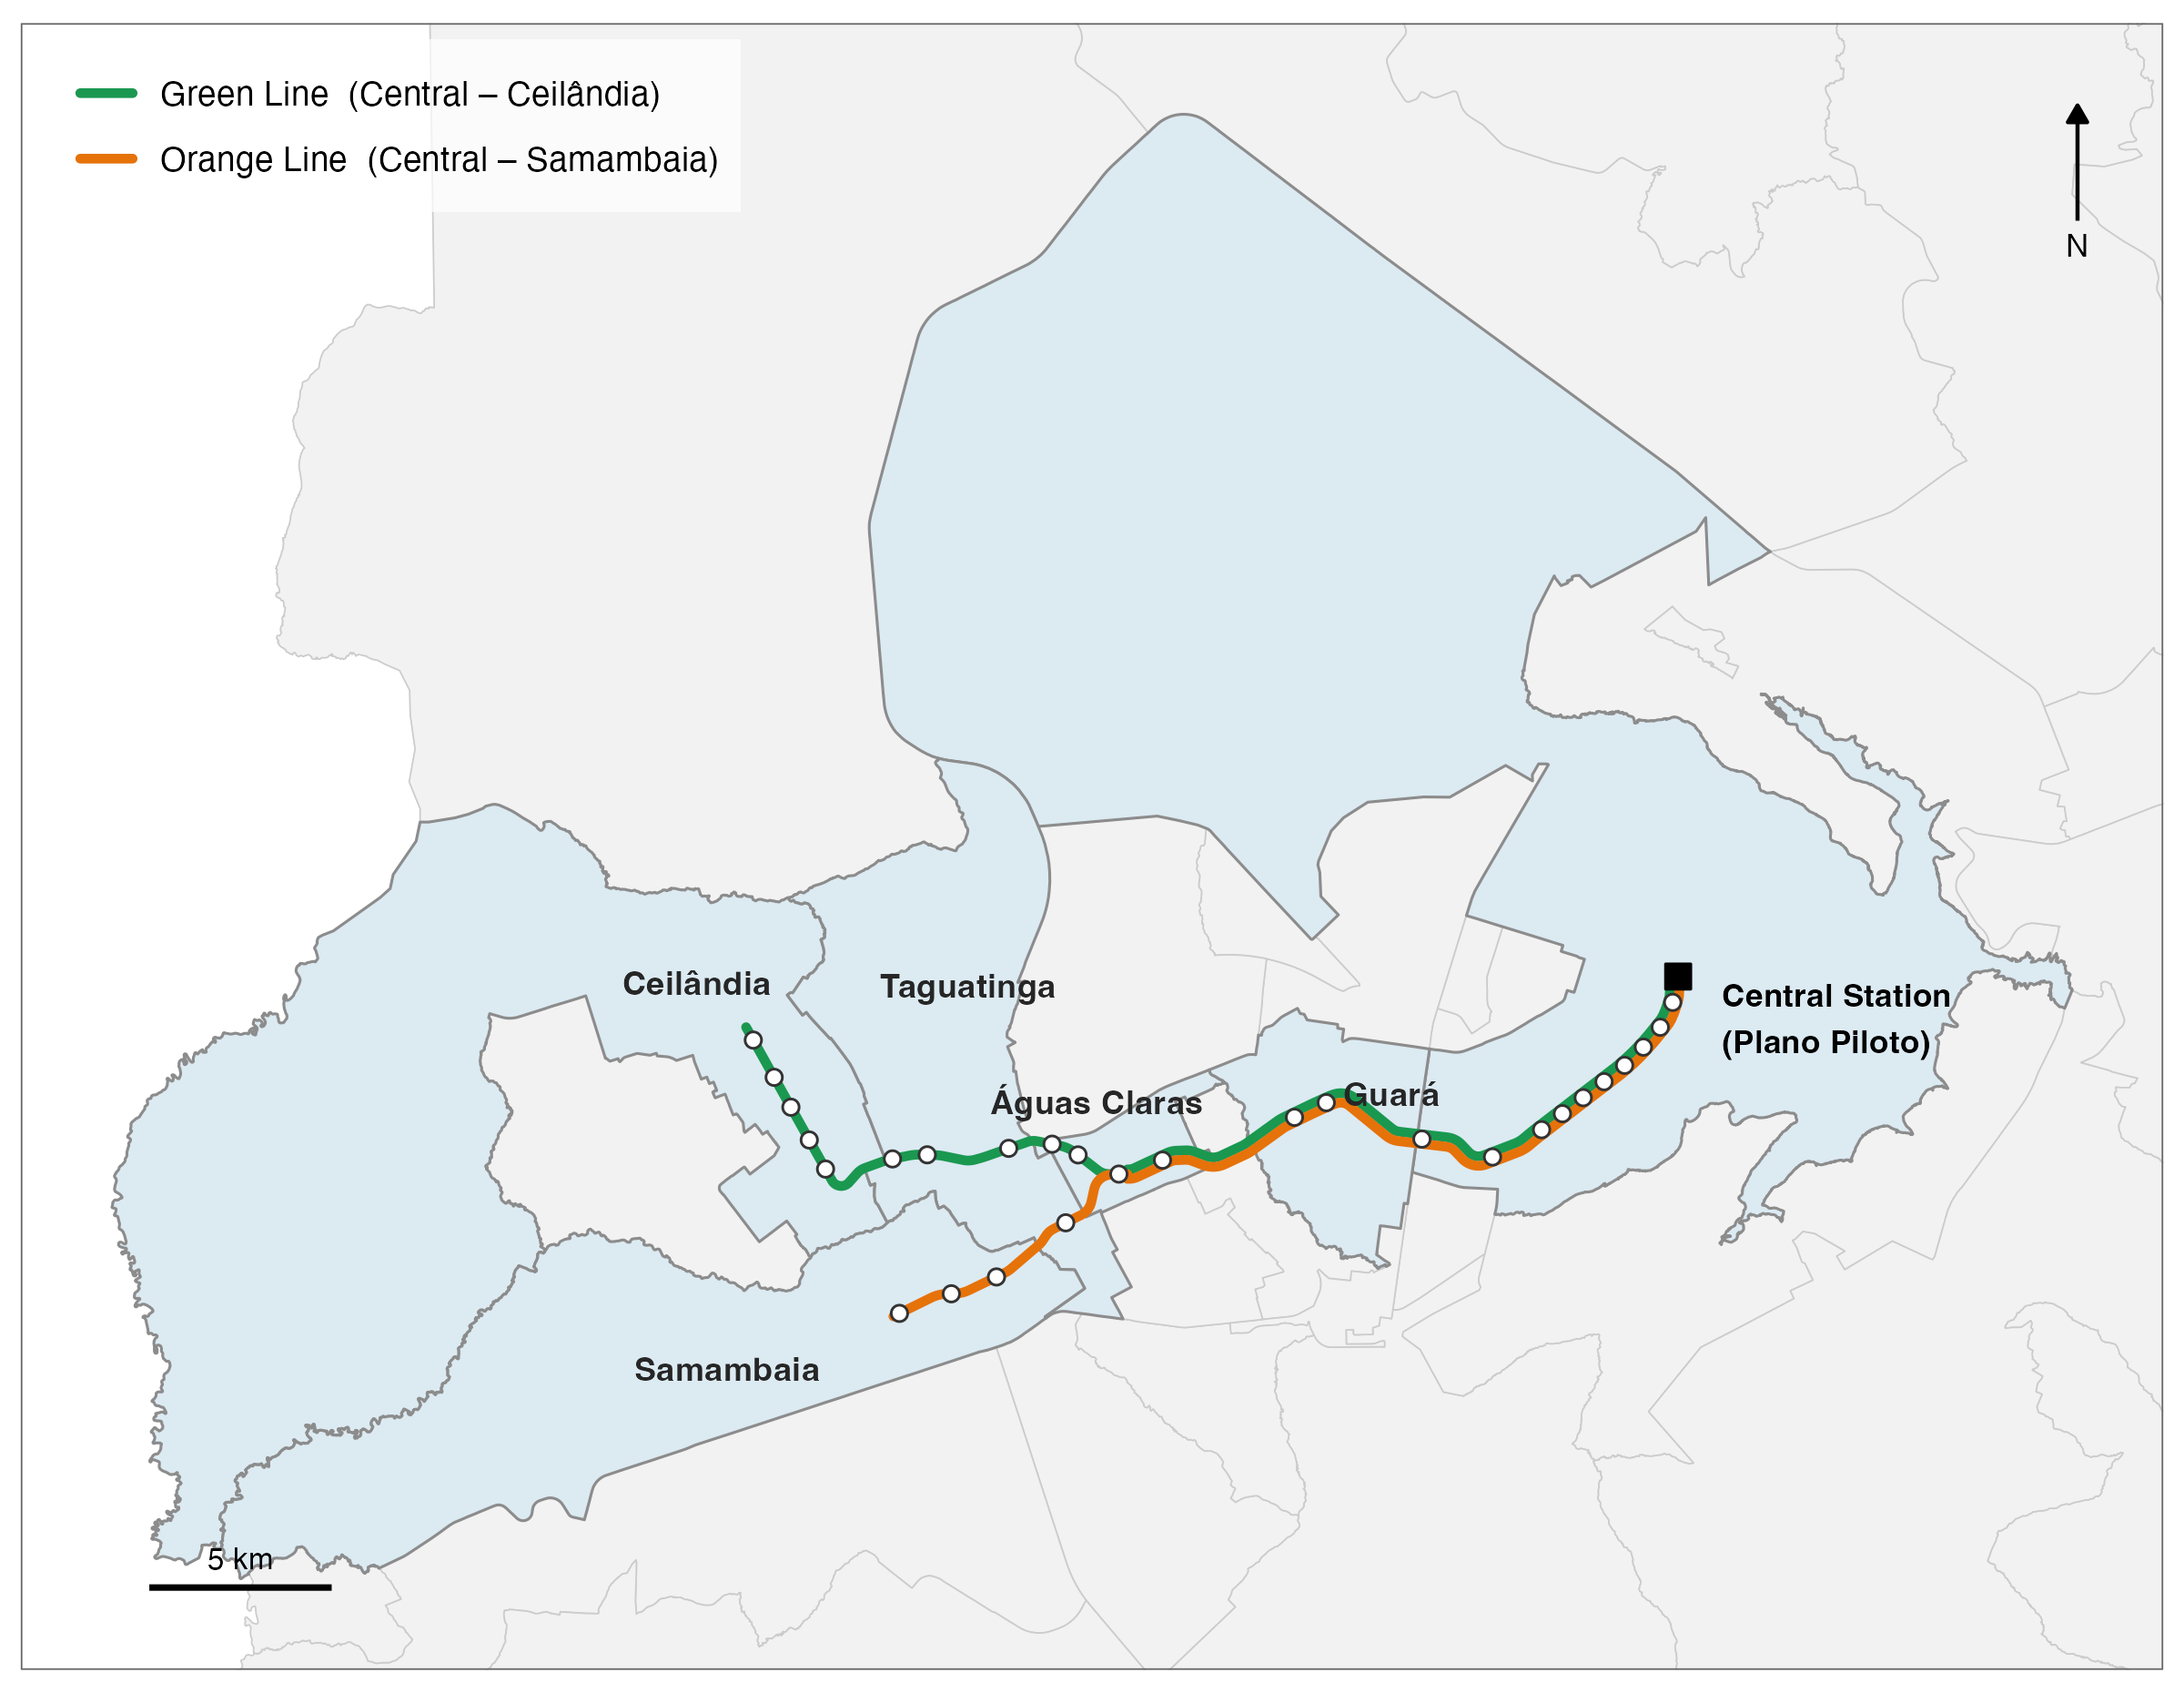
\includegraphics[width=0.92\textwidth]{images/subway_system_bsb.png}
\vspace{-0.2cm}
\begin{flushleft}
\footnotesize \textit{Note}: The map shows the two operating lines of the Brasília subway system, their stations, and the six administrative regions (RAs) served by the network, identified by name. The Green Line links Central station---located at the \textit{Plano Piloto} bus terminal, in Brasília's employment core---to Ceilândia, and the Orange Line branches toward Samambaia; both lines share the central trunk and bifurcate near Taguatinga. Highlighted polygons indicate the served RAs; remaining RAs of the Federal District are shown in grey for context. Coordinates are in SIRGAS 2000 / UTM zone 23S. \textit{Source}: Brasília GeoPortal (GeoPortal/DF); authors' elaboration.
\end{flushleft}
\end{figure}

This spatial configuration is precisely what makes the system relevant to the question studied in this paper. Brasília's employment and public services remain heavily concentrated in the legally protected \textit{Plano Piloto}, while most of the population resides in distant satellite cities, a separation between residence and workplace that is actively maintained by the city's land-use regime \citep{de2025evolution}.\footnote{See also \citep{codeplan2018expansao} on the socioeconomic profile of the subway's direct area of influence.} By connecting lower-income peripheral regions such as Ceilândia, Samambaia, and Taguatinga to the central labor market, the subway would operate as a labor-market access shock for the residents of exposed areas. The scale of this connection is non-trivial: the system carried approximately 42.5 million passengers in 2024, an average of about 3.5 million per month and on the order of 148,000 passengers on a typical weekday, with Central station, at the \textit{Plano Piloto} bus terminal, by far the busiest node in the network.\footnote{Ridership figures are reported in the \href{https://agenciabrasilia.df.gov.br/w/metro-df-passa-dos-425-milhoes-de-passageiros-ao-ano-e-projeta-ampliacao-para-2025/}{Metrô-DF Annual Administration Report for 2024} and in associated official communications of the Federal District government.}

For the purposes of identification, the most relevant feature of this history is the existence of a planned but unbuilt alignment. The 1986--1987 IMT feasibility study produced a network design that was set aside in favor of subsequent studies and was never implemented. The historical record does not provide a public, definitive explanation for why the IMT proposal was discarded. Several factors plausibly contributed and are consistent with the documented sequence of events: the change of state administration between the design's completion and the eventual construction phase; the financing difficulties that surrounded the project throughout the late 1980s and early 1990s; and a technical reassessment of the system's design, including its mode and alignment. The available evidence suggests that the abandonment reflected the institutional and political circumstances of the period rather than the income trajectories of individual census tracts---an assumption that is central to the instrumental-variable strategy developed in Section~\ref{s:methodology}, which uses proximity to this discarded alignment as an instrument for realized subway exposure.

\section{Data and Summary Statistics}
\label{s:data}

To investigate the effects of the construction of Brasília's subway system on its citizens income, we use geographic and socioeconomic data from the Brazilian Institute of Geography and Statistics (IBGE). Specifically, we use census-tract data for Brasília from the 2000 and 2010 censuses.\footnote{Brazil's census happens once every ten years. The 1980 and 1991 censuses are not used because neither provides micro-geographic data disaggregated at the census-tract level, making pre-trend analysis at this level of spatial resolution infeasible.} Our main outcome is tract-level per capita income and its change over 2000--2010. Per capita income is constructed, for each census tract and year, as the ratio of the sum of nominal monthly income declared by household heads to the total number of residents in permanent private dwellings.\footnote{The numerator captures only the income declared by the household head, not the total income of all residents. This restriction is data-driven: the 2000 Census does not publish total income of all persons in the universe of census tracts, providing only income distributions by bracket. Two features support the validity of this measure for the purposes of this study. First, since the numerator is defined identically in both years, any systematic underestimation cancels in the 2000--2010 log difference, preserving the interpretation of the coefficient as relative income growth. Second, household heads are more likely than other household members to be long-term, stable residents of the same census tract across both census years. Changes in the head's income between 2000 and 2010 therefore more plausibly reflect genuine earnings improvements for incumbent residents---those who were already living in the tract before and after subway access---rather than compositional change driven by new, higher-income arrivals. This aligns directly with the real income gains interpretation pursued in this study. Any additional income gains accruing to other household members are not captured, so the estimates constitute a lower bound on the total household income effect of subway access.} We also use baseline (2000) tract characteristics as controls: distance to Brasília's CBD, population, the share with completed higher education, the illiteracy rate, and the share of residents aged 65+. The reason why we focus on these two years is because Brasília's subway system began operating in 2001, meaning we have data from before and after the subway's implementation. Data for the subway lines and stations, as well as the geographic boundaries the Administrative Regions,\footnote{The Federal District (DF) has no municipalities; it is divided into Administrative Regions (Regiões Administrativas, RAs), subdistrict units used for local public administration and statistical reporting.} were obtained from the Brasília GeoPortal (GeoPortal/DF), which provides cartographic and urban-planning information for the capital. For the instrumentation of Brasília's subway system we use the abandoned (planned but not built) project sketch produced by the Mauá Institute of Technology.

The 2000 and 2010 Censuses use different census-tract boundaries: in 2010, many 2000 tracts were split (subdivided), meaning the original polygon was divided into two or more smaller polygons. To make the statistical analyses in this study feasible, we harmonize the 2010 census-tract map with the 2000 census-tract map; the formal details of this procedure are described in Appendix~\ref{s:appendix_harmonization}.

Our analysis focuses on census tracts located within a 10 km radius of the nearest subway station. This restriction is motivated by comparability: tracts far from the subway network are likely to differ systematically from those plausibly affected by the subway system in terms of urban form, land-use regulation, baseline socioeconomic conditions, and broader patterns of development. By limiting the sample to a relatively narrow band around the subway network, we compare ``treated'' tracts (those closer to stations) to ``control'' tracts that are geographically proximate and embedded in the same metropolitan context, reducing concerns that estimated differences in income dynamics are driven by large-scale spatial heterogeneity rather than by subway access. To define exposure, we classify a tract as treated if it lies within 1 km of the nearest subway station. This choice follows the Institute for Transportation and Development Policy (ITDP) \emph{People Near Transit} metric, which adopts a 1 km radius to capture the maximum distance most users are willing to walk to access metro service \citep{marks2016people}. This threshold corresponds roughly to a 10--15 minute walk and is widely used in the empirical literature as a reasonable catchment area for mass transit stations \citep{iamtrakul2024exploring, yang2024does, mohammad2017effect}. Given this localized nature of accessibility gains, restricting the estimation sample to tracts within 10 km of a station helps ensure that the control group consists of locations for which the subway is at most a marginal amenity, strengthening the credibility of the counterfactual. Figure~\ref{fig:1} reports the spatial distribution of census tracts and subway infrastructure in Brasília for 2000 and 2010 with harmonized census tracts.

\begin{figure}[h!]
\caption{Spatial Distribution of Census Tracts and Subway Infrastructure in Brasília}
\label{fig2a}
\vspace{-0.4cm}
    \centering
    \begin{subfigure}[b]{0.49\textwidth}
        \centering
        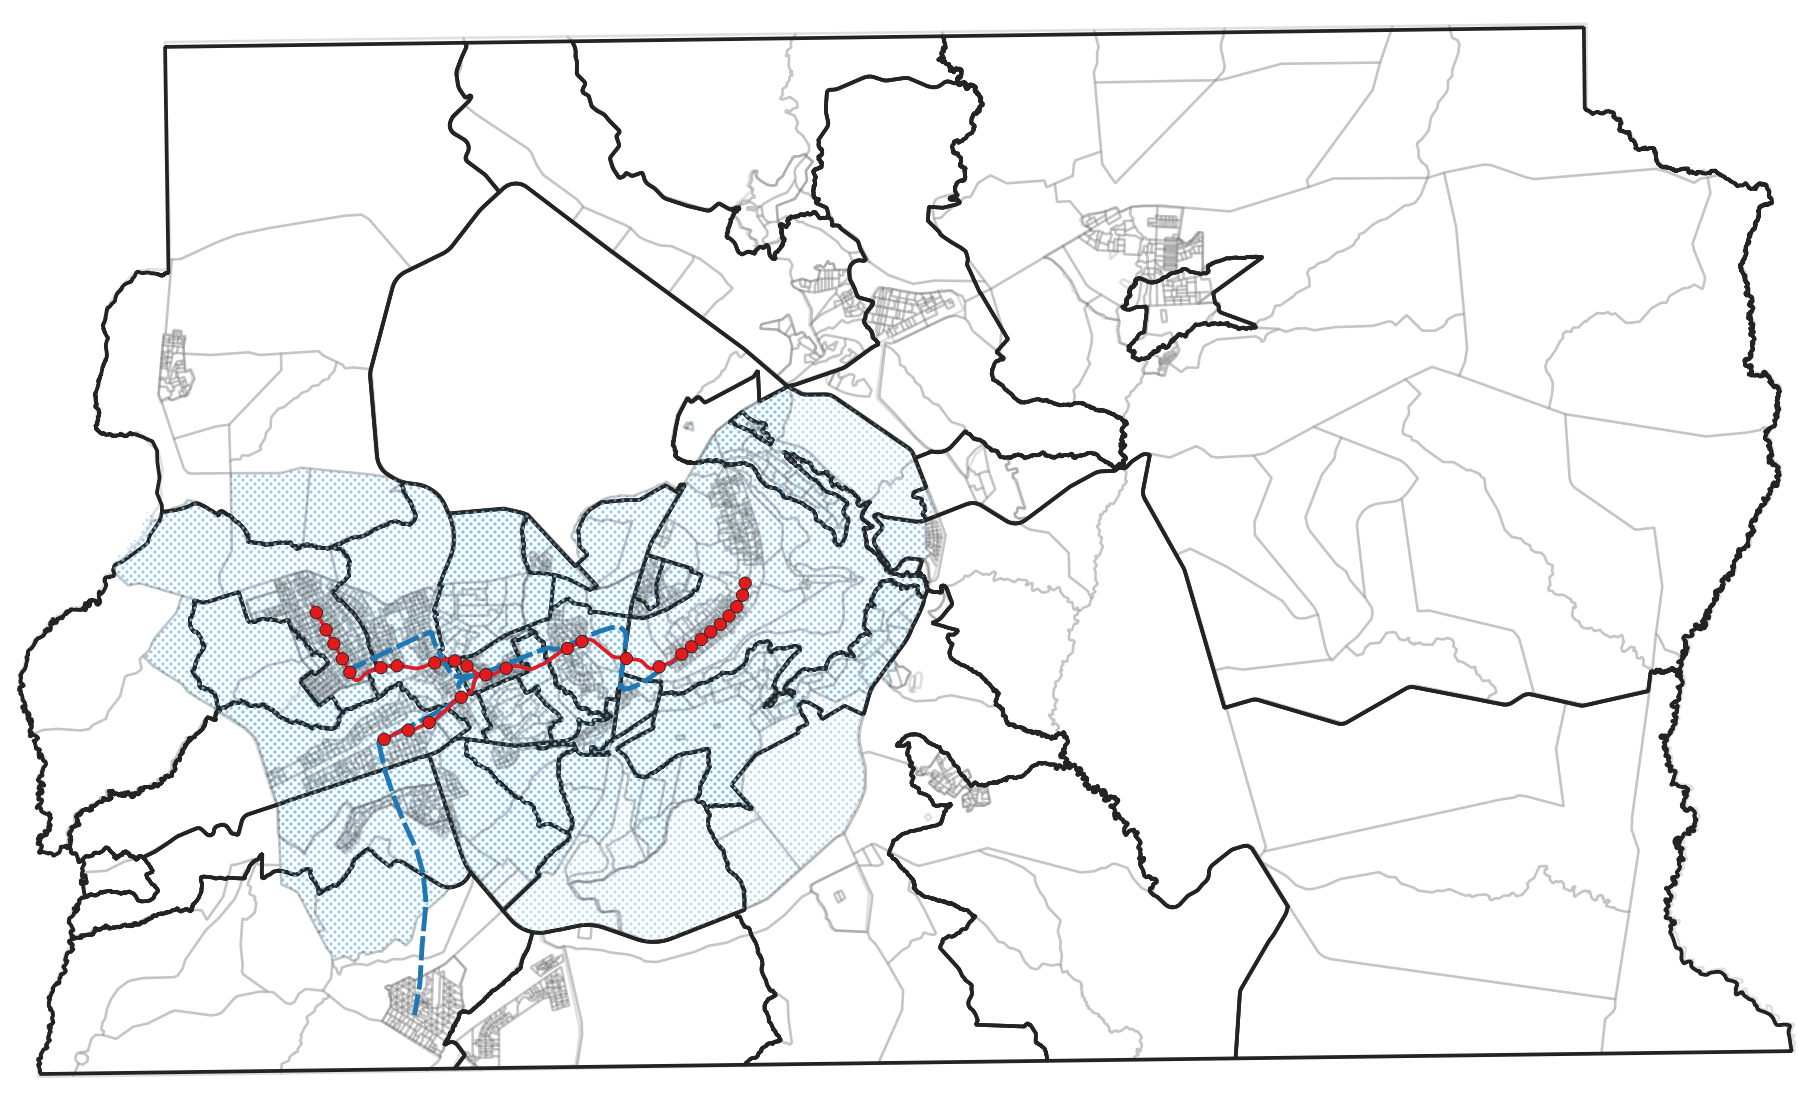
\includegraphics[width=\textwidth]{images/bsb2000.png}
        \caption{\footnotesize Census tracts (2000), subway lines (built and planned) and stations, Administrative Regions, and 10 km buffer.}
    \end{subfigure}
    \hfill
    \begin{subfigure}[b]{0.49\textwidth}
        \centering
        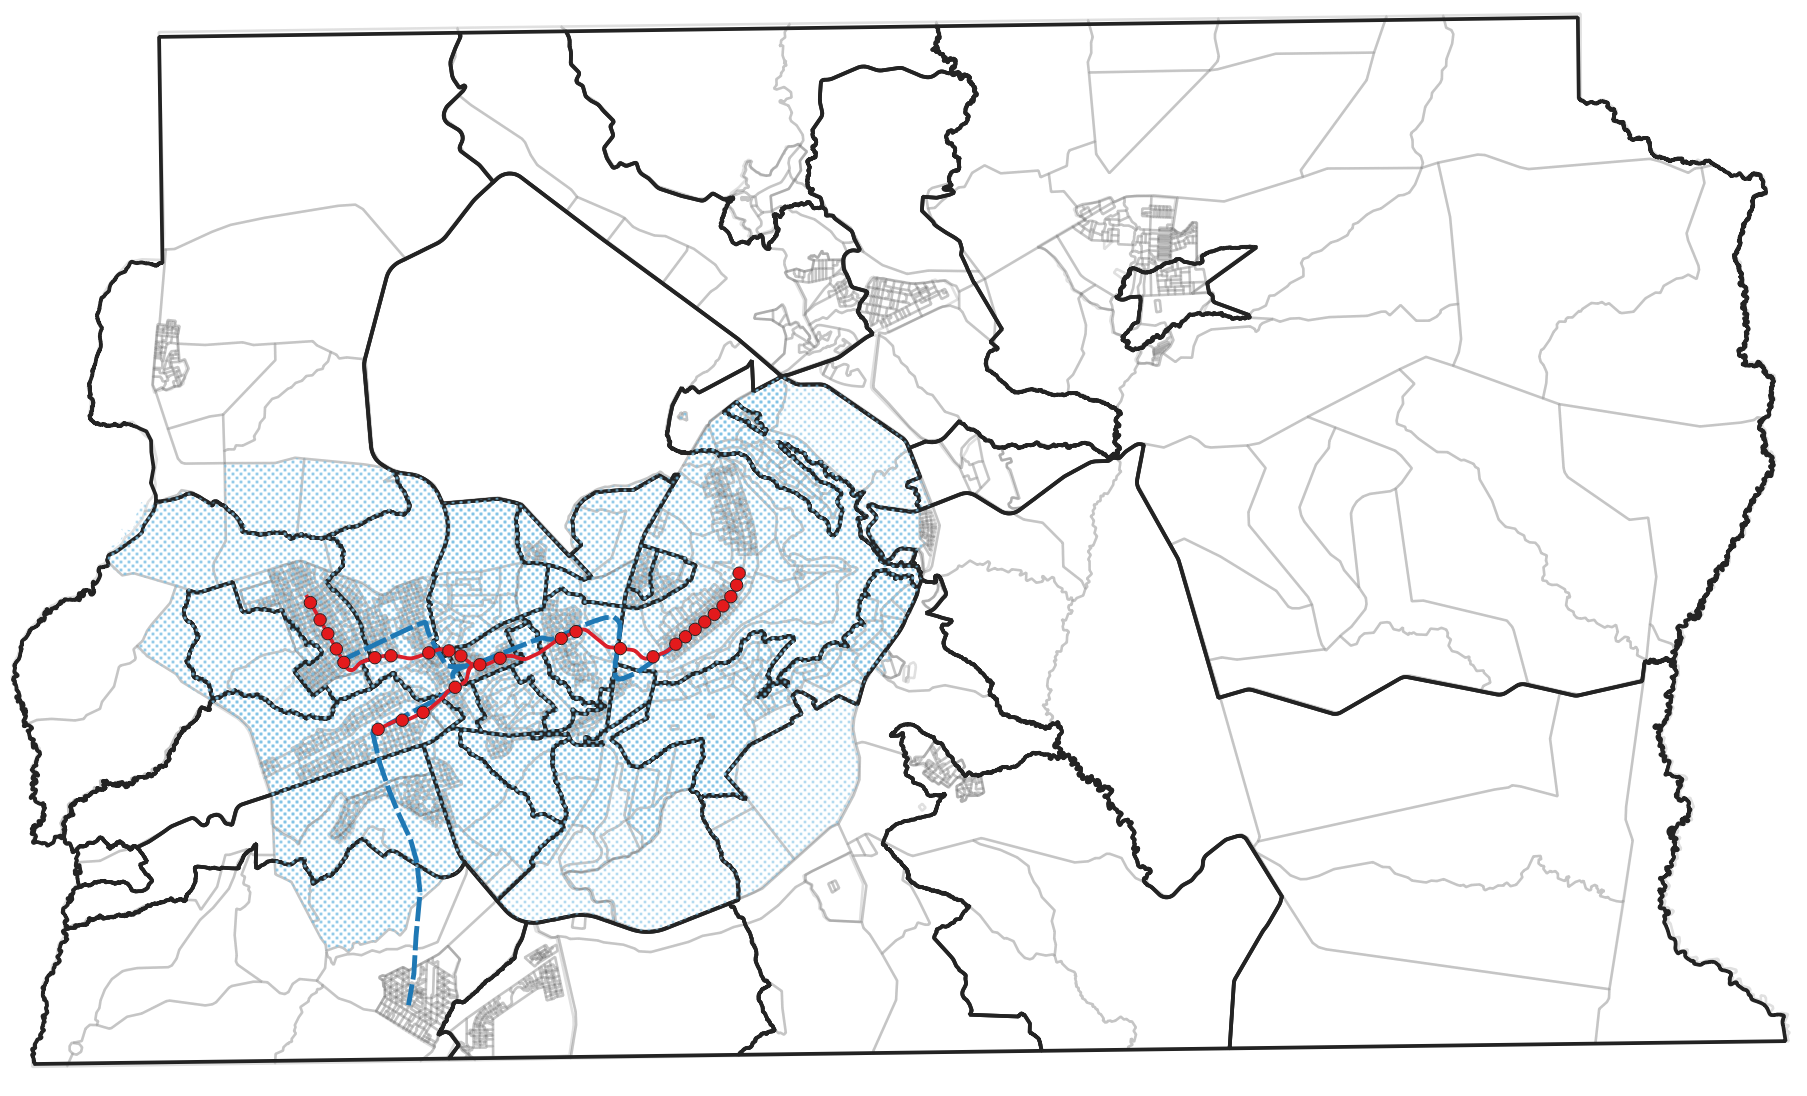
\includegraphics[width=\textwidth]{images/bsb2010.png}
        \caption{\footnotesize Harmonized census tracts (2010), subway lines (built and planned) and stations, Administrative Regions, and 10 km buffer.}
    \end{subfigure}
    \label{fig:1}
\end{figure}

Table~\ref{tab:descriptive} reports summary statistics separately for exposed ($\leq 1$ km from the nearest station) and non-exposed ($>1$ km) census tracts in 2000 and 2010.\footnote{Some demographic and educational composition variables were not reported in the 2010 Census extracts used in this study. This is not a concern for our empirical strategy, since these variables enter the regressions only as baseline (2000) controls.} Of the 1,860 tracts within 10 km of the network in 2000, 592 (32\%) are classified as exposed and 1,268 (68\%) as non-exposed. In 2000, exposed tracts had a higher mean per capita income (R\$618 vs.\ R\$470) and a lower illiteracy rate (5.5\% vs.\ 6.9\%), consistent with subway stations being located in relatively established urban areas. Both groups experienced substantial nominal income growth between 2000 and 2010 (exposed: R\$618 to R\$1{,}388; non-exposed: R\$470 to R\$1{,}035), reflecting the broad-based income expansion observed throughout Brazil in this period. The raw difference in growth rates between the two groups is modest, which highlights why a causal identification strategy is necessary: unconditional comparisons confound the effect of subway access with pre-existing differences in tract characteristics and common income trends.

\begin{table}[!h]
\centering
\caption{Descriptive statistics by subway exposure --- census tracts within 10 km (2000 and 2010)}
\label{tab:descriptive}
\resizebox{0.7\textwidth}{!}{%
\begin{tabular}{lcccc}
\toprule
 & \multicolumn{2}{c}{Exposed ($\leq$ 1 km)} & \multicolumn{2}{c}{Non-exposed ($>$ 1 km)} \\
\cmidrule(lr){2-3}\cmidrule(lr){4-5}
 & 2000 & 2010 & 2000 & 2010 \\
Number of tracts & 592 & 618 & 1,268 & 1,269 \\
\midrule
\multicolumn{5}{l}{\textit{Panel A: Outcome}} \\[2pt]
Per capita income (R\$) & 618 & 1{,}388 & 470 & 1{,}035 \\
 & (569) & (1{,}060) & (521) & (1{,}046) \\[4pt]
\midrule
\multicolumn{5}{l}{\textit{Panel B: Geographic controls}} \\[2pt]
Distance to CBD (meters) & 16{,}367 & --- & 17{,}234 & --- \\
 & (7{,}686) &   & (8{,}522) &  \\[4pt]
Distance to nearest road (meters) & 1{,}141 & --- & 941 & --- \\
 & (816) &   & (719) &  \\[4pt]
\midrule
\multicolumn{5}{l}{\textit{Panel C: Socioeconomic baseline (2000)}} \\[2pt]
Population & 706 & 712 & 816 & 1{,}024 \\
 & (289) & (975) & (298) & (1{,}708) \\[4pt]
Share of illiterate residents & 0.055 & --- & 0.069 & --- \\
 & (0.055) &   & (0.050) &  \\[4pt]
Share with college degree & 0.015 & --- & 0.012 & --- \\
 & (0.024) &   & (0.025) &  \\[4pt]
Share aged 65 or older & 0.049 & --- & 0.034 & --- \\
 & (0.036) &   & (0.025) &  \\[4pt]
\bottomrule
\end{tabular}%
}
\scriptsize
\begin{flushleft}
\textit{Note}: Standard deviations in parentheses. Exposed tracts lie within 1 km of the nearest subway station; non-exposed tracts lie between 1 km and 10 km. Geographic and socioeconomic variables enter the regressions as 2000 baseline characteristics. Statistics for 2010 are not reported for variables not available in the 2010 Census extracts. The number of tracts differs between the two census years because 63 of the 1,905 tracts within 10 km appear in only one of the censuses (45 only in 2010, 18 only in 2000); the regressions use tracts observed in both years.
\end{flushleft}
\end{table}


\section{Methodology}
\label{s:methodology}

The analysis measures the impact of the Brasília Subway System on local economic outcomes at census-tract level. The main outcome is income growth, defined as the change in (log) per-capita income between 2000 and 2010. Let $i$ index census tracts and let $r(i)$ denote the administrative region (Região Administrativa, RA) to which tract $i$ belongs. The dependent variable is constructed as a cross-section of changes\footnote{A ``cross-section of changes'' means that each tract appears once in the regression, with its outcome already expressed as the 2000-2010 change. This differs from a panel specification (which would stack observations for 2000 and 2010 and include time variation explicitly). In our specification, the time dimension is absorbed into the construction of $\Delta y_{i}$.}:
\begin{equation}
    \Delta y_{i} \equiv \log (\text{income}_{i,2010}) - \log (\text{income}_{i,2000})
    \label{eq:incomechange}
\end{equation}

Let $D_{i}$ denote exposure to the subway. Subway exposure is defined using geographic proximity to stations. For each census tract $i$, let $d_{i}$ denote the Euclidean distance (in meters) from the tract (its centroid) to the nearest subway station open at the time of the 2010 Census. The baseline exposure indicator classifies a tract as treated if it lies within 1,000 meters of the nearest station:
\begin{equation}
    D_{i} \equiv 1\{d_{i} \leq 1000\}
    \label{eq:exposure_var}
\end{equation}
thus a tract is classified as exposed ($D_{i} = 1$) if it lies within 1,000 meters of the nearest station, and unexposed ($D_{i} = 0$) otherwise.\footnote{This threshold follows the Institute for Transportation and Development Policy (ITDP) \emph{People Near Transit} metric and corresponds roughly to a 10--15 minute walk, as discussed in Section~\ref{s:data}.} 

A central concern is that subway placement is endogenous: lines and stations may have been located in areas with different pre-trends, political priorities, or expected growth. To address this, the empirical strategy uses two-stage least squares (2SLS). The instrument $Z_{i}$ is based on a discarded/planned subway project (the ``counterfactual'' design), capturing intended network placement that was not fully implemented.\footnote{The planned-project instrument is constructed as a binary proximity measure, analogous to the realized exposure. Because planned station locations are not available, planned access is derived from the minimum distance between the census-tract centroid and the closest segment of the planned (discarded) subway alignment. The instrument equals one if this distance is below 1,000 meters and zero otherwise, matching the treatment threshold. This represents a departure from the realized exposure variable, which is defined using distance to the nearest station rather than to the nearest line segment. The asymmetry introduces classical measurement error into the instrument: $Z_{i}$ is a noisy proxy for the latent concept of planned station proximity, which attenuates the first-stage coefficient and biases the 2SLS estimates toward zero. The estimated income effects should therefore be interpreted as a lower bound on the true causal effect.} The exclusion restriction requires that proximity to the IMT alignment affects income growth only through realized subway access, and not through any independent channel. The defense of this assumption rests on three arguments.

The first argument is temporal. The IMT alignment was designed in 1986--1987, more than a decade before the baseline year of this study (2000) and nearly a quarter century before the end of the outcome period (2010). Income growth trajectories at the census-tract level between 2000 and 2010 could not have influenced a planning document drafted in the mid-1980s: reverse causality is ruled out by construction. This approach follows an established strategy in the empirical literature on urban transportation \citep{baumsnow2007highways, severen2023commuting, mayertrevien2017largescale, brinkman2024freeway}: network plans drawn to address the conditions of their era are used to isolate the causal effects of infrastructure on later outcomes, precisely because the fundamentals that shaped the plan---population distribution, transport connectivity, and topography as they existed at the time of planning---predate the outcome dynamics of interest.

The second argument concerns the reasons why the IMT plan was never implemented. A plan that predates the outcome still needs to be abandoned for reasons unrelated to subsequent income growth. In the Brasília case, the available evidence points to three institutional factors: a change of state administration between the completion of the IMT study in early 1987 and the eventual construction phase that began in 1992; the severe financing constraints of the period, marked by hyperinflation and contested federal transfers; and a technical reassessment of the system's mode and alignment by the incoming administration. None of these factors is plausibly linked to the income trajectories of specific census tracts over the 2000--2010 decade. This mirrors the pattern documented in the closest analogues in the literature: \cite{mayertrevien2017largescale} show that the Paris RER plan diverged from its initial design following a political transition and budgetary pressures, and \cite{brinkman2024freeway} document that U.S. freeway construction departed from initial plans due to organized community opposition and subsequent regulatory changes---in both cases, the divergence reflects factors that are unrelated to the neighborhood-level outcomes being estimated.

The third argument addresses the geographic overlap between the IMT alignment and the realized network. Both proposals were designed to connect the \textit{Plano Piloto} to the same peripheral administrative regions, so some similarity in their general corridor is expected and does not invalidate the instrument. What matters for identification is not that the two alignments are distinct at the corridor level, but that the specific tracts classified as treated differ between them, and that these differences arise from routing decisions unrelated to income growth.\footnote{The data confirm this. Among the 1,887 tracts within 10~km of a station, the realized treatment and the planned instrument disagree for 16.2\% of tracts: 21\% of treated tracts fall outside the instrument and 28\% of instrument-exposed tracts are untreated. The two indicators are correlated at 0.64, leaving ample independent variation, which the strong first stage confirms is informative (the bivariate first-stage $F$-statistic is about 1{,}284; with administrative-region fixed effects and controls, the first-stage $F$-statistics in Table~\ref{tab:iv_results} range from 733 to 816).} A tract may fall within 1,000 meters of the IMT alignment but outside that range from the realized network, or the reverse, depending on the local routing choices of each design. Those differences---a curve adjusted for topography, a segment rerouted after a change in technical criteria---reflect the administrative and engineering decisions of 1986--1987, not the income trajectory of the tracts involved.

The IV strategy thus relies on (i) instrument relevance, i.e., planned exposure $Z_{i}^{(k)}$ must predict realized exposure $D_{i}^{(k)}$; this is assessed using the first-stage F-statistic; and (ii) the exclusion restriction, namely that---conditional on baseline covariates $X'_{i,2000}$ and administrative-region fixed effects $\alpha_{r(i)}$---planned exposure affects income growth only through realized subway exposure. The 2SLS coefficient $\beta_{1}$ is interpreted as a local average treatment effect (LATE) for census tracts whose realized exposure is shifted by the planned alignment. As we discussed in Section~\ref{s:data}, the preferred specification restricts the sample to tracts within 10 km of the nearest subway station to improve comparability among nearby neighborhoods.

The estimation is carried out via 2SLS with administrative-region (RA) fixed effects. The first-stage equation is:
\begin{align}
    D_{i}^{(k)} &= \pi_{0} + \pi_{1}Z_{i}^{(k)} + X'_{i,2000}\vartheta + \alpha_{r(i)} + u_{i}, \label{eq:first_stage_rafe}
\end{align}
where $D_{i}^{(k)} \in \{0,1\}$ is the binary subway exposure indicator that equals one if tract $i$ lies within $k$ meters of the nearest station and zero otherwise; $Z_{i}^{(k)} \in \{0,1\}$ is the corresponding binary instrument constructed from the planned/discarded network (defined analogously for the same threshold $k$); $X'_{i,2000}$ is the vector of baseline covariates (log distance to Brasília's center in 2000, log distance to the nearest highway in 2000, share of household heads with completed higher education in 2000, illiteracy share in 2000, share aged 65$+$ in 2000, log per-capita income in 2000 and log population in 2000); and $\alpha_{r(i)}$ are RA fixed effects. The fitted values from \eqref{eq:first_stage_rafe}, $\hat{D}_{i}^{(k)}$, capture the component of realized subway exposure explained by the planned/discarded network, conditional on baseline covariates and RA-level unobservables.

The second-stage equation is:
\begin{align}
    \Delta y_{i} &= \beta_{0} + \beta_{1} \hat{D}_{i}^{(k)} + X'_{i,2000}\gamma + \alpha_{r(i)} + \varepsilon_{i}, \label{eq:second_stage_rafe}
\end{align}
where $\Delta y_{i}$ is income growth from 2000 to 2010. This equation relates medium-run income growth across census tracts to \emph{predicted} subway exposure, purged of endogenous placement decisions through the instrumental-variable strategy. The coefficient of interest, $\beta_{1}$, measures the causal effect of being exposed to the subway system—within distance threshold $k$—on income growth over the 2000--2010 decade, using only variation in exposure induced by the planned/discarded network. As a result, $\beta_{1}$ captures how income growth differs between tracts that became effectively exposed to the subway and otherwise similar tracts that did not, holding constant baseline socioeconomic characteristics and unobserved RA-level factors. In other words, the estimation assesses whether census tracts exposed to the subway experienced a larger (or smaller) positive change in income over the decade relative to non-exposed tracts.

Administrative-region fixed effects are included to absorb unobserved factors that are common to all census tracts within the same Região Administrativa (RA) and that may systematically affect income growth between 2000 and 2010. Even though the dependent variable is a change $\Delta y_{i}$, different RAs can follow different average growth paths over the decade due to persistent differences in local public services, land-use regulation, infrastructure provision, labor-market conditions, and broader neighborhood amenities. By adding RA fixed effects, identification comes from comparing more and less subway-exposed tracts within the same RA, reducing bias from cross-RA differences that could otherwise be correlated with subway placement or with the planned-network instrument. Year fixed effects are not included, as the specification is estimated in long differences.\footnote{A long-differences specification collapses the time dimension into the outcome variable, expressing the dependent variable as the change between two periods. With a single cross-section of changes, a year fixed effect would be mechanically collinear and therefore redundant.}

Standard errors are clustered at the RA level. Clustering at the RA level allows for arbitrary correlation in unobserved factors within administrative regions, which is appropriate given that tracts in the same RA share common policies and local conditions.


\section{Subway's Effect on Income Growth}
\label{s:results}

In this section, we present the empirical results of the analysis using the instrumental-variable strategy described in Section~\ref{s:methodology}. We begin by reporting the main results on the effect of subway exposure on income growth.  We then present a series of robustness checks designed to assess the stability of the estimates under alternative specifications, samples, and identification assumptions.

\subsection{Main Results}
\label{s:results1}

Table \ref{tab:iv_results} reports the second-stage 2SLS estimates of the effect of subway exposure on census-tract income growth between 2000 and 2010. All specifications treat subway exposure as endogenous and instrument it using the corresponding planned/discarded network proximity indicator at the same distance threshold. The sample is restricted to census tracts located within 10 km of the subway network, and all regressions include administrative-region (RA) fixed effects, with standard errors clustered at the RA level.

Column (1) presents the baseline specification, which includes only the initial level of income, measured as log per-capita income in 2000. Including the baseline income level is essential in this context because the dependent variable is income growth over the subsequent decade. Areas with higher initial income tend to exhibit lower subsequent growth due to convergence or mean-reversion dynamics, while poorer areas may experience faster relative growth. Omitting baseline income would therefore confound the estimated effect of subway exposure with these underlying growth dynamics, potentially attributing to the subway what is in fact a catch-up process across neighborhoods. Column (2) adds geographic controls that capture broader accessibility patterns in the urban structure: the logarithm of the distance to Brasília's CBD and the logarithm of the distance to the nearest highway. Since Brasília's subway system lines largely follow major transport corridors, this control help ensure that the subway exposure variable captures the specific contribution of rail access rather than general road-based accessibility. Distance to the CBD is included because income tends to decline with distance from the center, and the subway radiates outward from that center. Without this control, the subway exposure variable could simply pick up the income premium of being central rather than the effect of rail access itself. Column (3) introduces a set of socioeconomic characteristics measured in 2000, including the share of residents with higher education, the illiteracy rate, the share of elderly residents (aged 65 or more), and population size. These variables proxy for differences in human capital, demographic structure, and settlement patterns that may influence income trajectories independently of transport infrastructure. Including these controls helps ensure that the estimated subway effect is not driven by pre-existing socioeconomic differences across neighborhoods. Finally, column (4) includes the full set of geographic and socioeconomic controls simultaneously. 

\begin{table}[htbp]
\centering
\caption{Effect of subway exposure on income growth: 2SLS first and second stage (10 km sample, 1,000 m threshold)}
\label{tab:iv_results}
\makebox[\textwidth][c]{\resizebox{0.85\textwidth}{!}{%
\begin{tabular}{lcccc}
\toprule
 & (1) & (2) & (3) & (4) \\
\midrule
\multicolumn{5}{l}{\textit{Panel A: First stage --- dep.\ var.: $D_i^{(1000)}$ (subway exposure indicator)}} \\[4pt]
Planned subway exposure $Z_i^{(1000)}$
  & 0.6118$^{***}$    & 0.6104$^{***}$    & 0.5922$^{***}$    & 0.5928$^{***}$ \\
  & (0.1112)          & (0.1158)          & (0.1015)          & (0.1055) \\[2pt]
\cmidrule(lr){1-5}
RMSE                            & 0.322 & 0.320 & 0.320 & 0.319 \\
Adjusted $R^2$                  & 0.488 & 0.491 & 0.493 & 0.495 \\
First-stage $F$-statistic       & 931.8 & 923.2 & 838.9 & 841.3 \\[2pt]
\midrule
\multicolumn{5}{l}{\textit{Panel B: Second stage --- dep.\ var.: $\Delta y_i$ (log per-capita income growth, 2000--2010)}} \\[4pt]
Fitted subway exposure
  & 0.1031$^{*}$      & 0.0935$^{*}$      & 0.1012$^{**}$     & 0.0952$^{**}$ \\
  & (0.0498)          & (0.0473)          & (0.0467)          & (0.0439) \\[4pt]
log(per-capita income, 2000)
  & $-$0.2961$^{***}$ & $-$0.3049$^{***}$ & $-$0.3327$^{***}$ & $-$0.3395$^{***}$ \\
  & (0.0476)          & (0.0467)          & (0.0333)          & (0.0327) \\[2pt]
\cmidrule(lr){1-5}
RMSE                            & 0.226 & 0.224 & 0.223 & 0.222 \\
Adjusted $R^2$                  & 0.290 & 0.296 & 0.305 & 0.310 \\
Administrative Region FE        & Yes      & Yes           & Yes              & Yes          \\
Controls                        & Baseline & + Geographic  & + Socioeconomic  & All controls \\
Observations                    & 1,692    & 1,692         & 1,692            & 1,692 \\
Wu--Hausman $p$-value           & $<0.001$ & $<0.001$      & $<0.001$         & $<0.001$ \\
\bottomrule
\end{tabular}
}} % closes \resizebox and \makebox
\begin{tablenotes}
\scriptsize
\item \textit{Notes:} Standard errors clustered at the administrative-region (RA) level in parentheses. Significance levels: $^{*}p<0.1$, $^{**}p<0.05$, $^{***}p<0.01$. All specifications include RA fixed effects and use the sample restricted to census tracts within 10 km of the subway network. Panel A reports the first-stage coefficient on the planned/discarded alignment indicator $Z_i^{(1000)}$; the first-stage $F$-statistic (reported within Panel A) tests instrument strength. Panel B reports the second-stage 2SLS coefficient on subway exposure. Wu--Hausman tests the null of exogeneity of subway exposure.
\end{tablenotes}
\end{table}

Panel A of Table~\ref{tab:iv_results} reports the first-stage estimates. The coefficient on the planned-network instrument $Z_i^{(1000)}$ is positive, large in magnitude (around 0.59--0.61), and highly statistically significant in all four specifications ($p < 0.001$), confirming that proximity to the planned/discarded alignment is a strong predictor of realized subway exposure. The first-stage $F$-statistics range from 839 to 932, well above conventional weak-instrument thresholds, providing strong evidence in favor of instrument relevance. Further support for the instrumental-variable approach comes from the Wu--Hausman test, which rejects the null of exogeneity of subway exposure in all specifications ($p < 0.001$), indicating that OLS estimates would be biased due to endogenous station placement. OLS estimates, reported in Appendix~\ref{s:appendix_ols} for comparison, are systematically smaller than their 2SLS counterparts, consistent with the endogeneity bias the IV strategy is designed to correct. Taken together, these results confirm that the 2SLS framework is appropriate and the instrument is both relevant and empirically justified.

Panel B of Table~\ref{tab:iv_results} presents the second-stage 2SLS estimates. Across all specifications, the coefficient on subway exposure is positive and statistically significant, indicating that census tracts located within 1,000 meters of the subway network experienced faster income growth between 2000 and 2010 relative to non-exposed areas. The estimated magnitude is highly stable across models, ranging from 0.0935 to 0.1031.\footnote{These estimates are best interpreted as a lower bound on the true causal effect. Because station locations for the discarded IMT alignment are unavailable, the instrument is constructed using distance to the nearest line segment rather than to the nearest station---introducing classical measurement error that attenuates the first-stage coefficient and biases the 2SLS estimates toward zero.} Importantly, the coefficient remains statistically significant as additional geographic and socioeconomic controls are introduced, suggesting that the positive relationship between subway exposure and income growth is not driven by observable differences in location or baseline socioeconomic characteristics.

Section~\ref{sub:results2} subjects the baseline estimates to a series of robustness tests. The first exercise varies the distance scope of the estimation sample (5 to 20 km), verifying that the results are not sensitive to how broadly the comparison group is drawn. The second varies the distance threshold used to define treatment (500 to 2,500 m), assessing whether the findings depend on any particular assumption about the walkable catchment area of a station. The third replaces the binary exposure indicator with continuous measures of proximity, assessing whether the results are robust to the functional form used to operationalize subway access. Two final checks address inference: one examines sensitivity to the level at which standard errors are clustered, and the other re-estimates the baseline using \citet{conley1999gmm} spatial standard errors to account for residual dependence across geographically proximate tracts.

\subsection{Robustness Tests}
\label{sub:results2}

\noindent
\textbf{Alternative Sample Radii.} Table~\ref{tab:iv_results_radius} reports 2SLS estimates across six alternative sample radii (5, 7.5, 10, 12.5, 15, and 20 km) holding all other aspects of the specification constant. In this exercise, the radius defines the full estimation sample---that is, both treated and control tracts must fall within the specified distance from the nearest subway station. The treatment indicator itself remains fixed at the 1,000 m threshold throughout; what varies is who enters the comparison group. The goal is to assess whether the baseline results are sensitive to how broadly the control group is drawn. If the estimates remain stable across radii, this constitutes evidence that the baseline finding is not an artifact of the particular 10 km cutoff.

\begin{table}[htbp]
\centering
\caption{Effect of subway exposure on income growth: 2SLS estimates across sample radii}
\label{tab:iv_results_radius}
\makebox[\textwidth][c]{\resizebox{0.85\textwidth}{!}{%
\begin{tabular}{lcccccc}
\toprule
\multicolumn{7}{c}{\textit{Dependent variable: log per-capita income growth (2000--2010)}} \\
\midrule
 & (1) & (2) & (3) & (4) & (5) & (6) \\
 & 5 km & 7.5 km & 10 km & 12.5 km & 15 km & 20 km \\
\midrule
Fitted subway exposure
  & 0.0998$^{**}$ & 0.0981$^{**}$ & 0.0952$^{**}$ & 0.0954$^{**}$ & 0.0982$^{**}$ & 0.0974$^{**}$ \\
  & (0.0411) & (0.0441) & (0.0439) & (0.0437) & (0.0439) & (0.0452) \\[4pt]

log(per-capita income, 2000)
  & $-$0.3509$^{***}$ & $-$0.3489$^{***}$ & $-$0.3395$^{***}$ & $-$0.3410$^{***}$ & $-$0.3419$^{***}$ & $-$0.3299$^{***}$ \\
  & (0.0355) & (0.0344) & (0.0327) & (0.0336) & (0.0326) & (0.0269) \\[4pt]
\midrule
Administrative Region FE & Yes & Yes & Yes & Yes & Yes & Yes \\
Observations             & 1,495 & 1,661 & 1,692 & 1,754 & 1,803 & 2,246 \\
RMSE                     & 0.221 & 0.220 & 0.222 & 0.221 & 0.222 & 0.219 \\
Adjusted $R^2$           & 0.293 & 0.312 & 0.310 & 0.314 & 0.312 & 0.305 \\
First-stage $F$-statistic& 716.3 & 815.6 & 841.3 & 872.4 & 869.1 & 946.6 \\
Wu--Hausman $p$-value    & 0.0005 & 0.0004 & 0.0006 & 0.0005 & 0.0004 & 0.0003 \\
\midrule
Instrument & \multicolumn{6}{c}{$Z_i^{(1000)}$} \\
\bottomrule
\end{tabular}
}}
\begin{tablenotes}
\scriptsize
\item \textit{Notes:} Standard errors clustered at the administrative-region (RA) level in parentheses. Significance levels: $^{*}p<0.1$, $^{**}p<0.05$, $^{***}p<0.01$. All specifications include RA fixed effects. Each column restricts the estimation sample to census tracts located within the indicated radius of the subway network. Subway exposure is treated as endogenous and instrumented by the planned/discarded network proximity indicator at the same 1,000 m threshold.
\end{tablenotes}
\end{table}

Results on Table~\ref{tab:iv_results_radius} are stable across all six sample definitions. The coefficient on subway exposure remains positive, statistically significant at the 5\% level, and virtually unchanged in magnitude across every radius tested, ranging narrowly from 0.095 to 0.100 with no systematic upward or downward trend as the sample expands. This stability directly addresses the concern motivating the exercise: the baseline finding is not an artifact of the particular 10 km cutoff. The standard errors also remain stable throughout, between 0.041 and 0.045, reflecting the fact that tracts added at wider radii are less informative controls, meaning they increase the sample size without proportionally reducing residual variance. The first-stage F-statistics and Wu--Hausman tests confirm that the instrumental-variable strategy remains valid under every sample definition considered. Taken together, these results confirm that the choice of 10 km as the baseline radius is conservative and well-grounded.
\vspace{0.75cm}

\noindent
\textbf{Alternative Distance Thresholds.} Table~\ref{tab:iv_results_threshold} reports 2SLS estimates across five alternative distance thresholds (500, 1,000, 1,500, 2,000, and 2,500 m) holding the estimation sample fixed at 10 km. While the previous subsection varied who enters the control group, this exercise varies who is classified as treated, testing whether the baseline results depend on any particular assumption about the walkable distance to the nearest subway station. If the estimated effect remains positive and consistent across thresholds, this constitutes evidence that the 1,000 m baseline cutoff does not mechanically produce the observed results.

\begin{table}[htbp]
\centering
\caption{Effect of subway exposure on income growth: 2SLS estimates across distance thresholds}
\label{tab:iv_results_threshold}
\makebox[\textwidth][c]{\resizebox{0.85\textwidth}{!}{%
\begin{tabular}{lccccc}
\toprule
\multicolumn{6}{c}{\textit{Dependent variable: log per-capita income growth (2000--2010)}} \\
\midrule
 & (1) & (2) & (3) & (4) & (5) \\
 & 500 m & 1000 m & 1500 m & 2000 m & 2500 m \\
\midrule

Fitted subway exposure
  & 0.0675 & 0.0952$^{**}$ & 0.0957$^{**}$ & 0.1296$^{*}$ & 0.1354 \\
  & (0.0570) & (0.0439) & (0.0433) & (0.0651) & (0.0953) \\[4pt]

log(per-capita income, 2000)
  & $-$0.3302$^{***}$ & $-$0.3395$^{***}$ & $-$0.3445$^{***}$ & $-$0.3485$^{***}$ & $-$0.3370$^{***}$ \\
  & (0.0338) & (0.0327) & (0.0363) & (0.0389) & (0.0376) \\[4pt]
\midrule
Administrative Region FE & Yes & Yes & Yes & Yes & Yes \\
Observations             & 1,692 & 1,692 & 1,692 & 1,692 & 1,692 \\
RMSE                     & 0.221 & 0.222 & 0.220 & 0.220 & 0.220 \\
Adjusted $R^2$           & 0.305 & 0.310 & 0.311 & 0.313 & 0.308 \\
First-stage $F$-statistic& 365.1 & 841.3 & 895.5 & 626.3 & 330.4 \\
Wu--Hausman $p$-value    & 0.097 & $<0.001$ & 0.043 & 0.012 & 0.065 \\
\midrule
Instrument & \multicolumn{5}{c}{$Z_i^{(k)}$} \\
\bottomrule
\end{tabular}
}}
\begin{tablenotes}
\scriptsize
\item \textit{Notes:} Standard errors clustered at the administrative-region (RA) level in parentheses. Significance levels: $^{*}p<0.1$, $^{**}p<0.05$, $^{***}p<0.01$. All specifications include RA fixed effects and use the sample restricted to census tracts within 10 km of the subway network. Subway exposure is treated as endogenous and instrumented by the planned/discarded network proximity indicator defined at each distance threshold.
\end{tablenotes}

\end{table}

Results from Table~\ref{tab:iv_results_threshold} are consistent with the baseline finding. The coefficient on subway exposure is positive across all five thresholds, ranging from 0.067 to 0.135, with no sign reversal, confirming that the estimated effect does not hinge on any particular definition of treatment. The intermediate thresholds, between 1,000 and 1,500 m, yield the most precise estimates, with the smallest standard errors and the largest first-stage F-statistics (841 and 895, respectively), and are the only specifications significant at the 5\% level; notably, the baseline specification sits exactly within this range. This pattern has a clear econometric explanation: at these distances there is sufficient variation between exposed and unexposed tracts within the same administrative region for the planned-network instrument to discriminate effectively between the two groups. At 500 m, fewer tracts are classified as treated, the instrument has less variation to exploit, and precision falls accordingly. At 2,000 and 2,500 m, point estimates are somewhat larger but considerably less precise, as the instrument loses strength at greater distances from the network. The 1,000 m baseline threshold therefore offers the best balance between instrument power, estimation precision, and economic interpretability. The overall pattern of positive and consistent estimates across all thresholds further strengthens the main results.
\vspace{0.75cm}

\noindent
\textbf{Continuous Measures of Exposure.} Table~\ref{tab:iv_results_intensity} reports 2SLS estimates that replace the binary exposure indicator with continuous treatment variables reflecting each tract's degree of proximity to the subway network. Three functional forms are considered, each capturing a different assumption about how accessibility declines with distance: a \textit{logistic sigmoid}, which maintains near-unity intensity up to the 1,000\,m transition zone and then falls off sharply, approximating the binary threshold with a smooth transition; a \textit{negative exponential}, which decays continuously from the station outward, assigning a steadily declining intensity to every tract without imposing any threshold; and a \textit{Gaussian kernel}, which concentrates most of its intensity within roughly one bandwidth of the station and decays much faster at larger distances.\footnote{The three specifications have the following functional forms. \textit{Logistic sigmoid}: $1\,/\bigl[1 + \exp\bigl((d_i - 1000)/\sigma\bigr)\bigr]$, where $\sigma$ governs the width of the transition zone around the 1,000\,m reference; for small $\sigma$ the function closely mimics the binary indicator, while larger values produce a progressively wider transition region. \textit{Negative exponential}: $\exp(-d_i/h)$, where $h$ is the decay parameter; the function reaches approximately $e^{-1} \approx 0.37$ of its maximum value at distance $h$. \textit{Gaussian kernel}: $\exp\!\bigl(-d_i^2/2\sigma^2\bigr)$, where $\sigma$ is the bandwidth. In all three cases, $d_i$ denotes the distance in meters from tract $i$'s centroid to the nearest subway station, and the instrument takes the same functional form applied to distance from the planned but unbuilt alignment. For each form, three bandwidth choices spanning a range from narrow to wide are reported to assess sensitivity to this parameter.} The instrument takes the same functional form applied to distance from the planned but unbuilt alignment.

\begin{table}[htbp]
\centering
\caption{Effect of subway exposure on income growth: 2SLS estimates with continuous treatment measures}
\label{tab:iv_results_intensity}
\makebox[\textwidth][c]{\resizebox{0.97\textwidth}{!}{%
\begin{tabular}{lrrr rrr rrr}
\toprule
\multicolumn{10}{c}{\textit{Dependent variable: $\Delta y_i$ (log per-capita income growth, 2000--2010)}} \\
\midrule
 & \multicolumn{3}{c}{\textit{Logistic sigmoid}} & \multicolumn{3}{c}{\textit{Negative exponential}} & \multicolumn{3}{c}{\textit{Gaussian kernel}} \\
\cmidrule(lr){2-4}\cmidrule(lr){5-7}\cmidrule(lr){8-10}
 & $\sigma\!=\!50$m & $\sigma\!=\!200$m & $\sigma\!=\!400$m
 & $h\!=\!750$m    & $h\!=\!1000$m    & $h\!=\!1500$m
 & $\sigma\!=\!700$m & $\sigma\!=\!900$m & $\sigma\!=\!1200$m \\
\midrule
Fitted subway exposure
  & 0.0968$^{**}$     & 0.1102$^{**}$     & 0.1396$^{*}$
  & 0.1614$^{*}$      & 0.1586$^{*}$      & 0.1577$^{*}$
  & 0.1200$^{*}$      & 0.1266$^{*}$      & 0.1331$^{*}$ \\
  & (0.0448)          & (0.0529)          & (0.0675)
  & (0.0880)          & (0.0839)          & (0.0852)
  & (0.0607)          & (0.0614)          & (0.0678) \\[4pt]
log(per-capita income, 2000)
  & $-$0.3402$^{***}$ & $-$0.3414$^{***}$ & $-$0.3429$^{***}$
  & $-$0.3382$^{***}$ & $-$0.3393$^{***}$ & $-$0.3394$^{***}$
  & $-$0.3401$^{***}$ & $-$0.3429$^{***}$ & $-$0.3436$^{***}$ \\
  & (0.0332)          & (0.0336)          & (0.0344)
  & (0.0338)          & (0.0341)          & (0.0344)
  & (0.0336)          & (0.0344)          & (0.0354) \\[4pt]
\midrule
Administrative Region FE  & \multicolumn{9}{c}{Yes} \\
Observations              & 1,692 & 1,692 & 1,692 & 1,692 & 1,692 & 1,692 & 1,692 & 1,692 & 1,692 \\
RMSE                      & 0.221 & 0.221 & 0.220 & 0.220 & 0.220 & 0.220 & 0.221 & 0.220 & 0.220 \\
Adjusted $R^2$            & 0.311 & 0.311 & 0.312 & 0.308 & 0.309 & 0.310 & 0.310 & 0.312 & 0.312 \\
First-stage $F$-statistic & 998.4 & 1281.1 & 1438.6 & 1132.5 & 1344.0 & 1569.8 & 1235.5 & 1433.2 & 1482.4 \\
Wu--Hausman $p$-value     & $<0.001$ & 0.002  & 0.005  & 0.033  & 0.030  & 0.045  & 0.005  & 0.005  & 0.015 \\
\bottomrule
\end{tabular}%
}}
\begin{tablenotes}
\scriptsize
\item \textit{Notes:} Standard errors clustered at the administrative-region (RA) level in parentheses. Significance levels: $^{*}p<0.1$, $^{**}p<0.05$, $^{***}p<0.01$. All specifications include RA fixed effects, all baseline controls, and use the sample restricted to census tracts within 10 km of the subway network. Three functional forms are used to operationalize subway proximity: logistic sigmoid $1/[1+\exp((d_i-1000)/\sigma)]$, where $\sigma$ governs the width of the transition zone around the 1,000\,m reference; negative exponential $\exp(-d_i/h)$, where $h$ is the decay half-life; and Gaussian kernel $\exp(-d_i^2/2\sigma^2)$, where $\sigma$ is the kernel bandwidth. For each form, the instrument applies the same function to distance from the planned but unbuilt alignment ($d_i^{\mathrm{proj}}$).
\end{tablenotes}
\end{table}

Table~\ref{tab:iv_results_intensity} confirms the main finding across all nine specifications. The coefficient on fitted subway exposure is positive and statistically significant in every case: at the 5\,\% level for the two narrower sigmoid bandwidths ($\sigma = 50$ and $200$\,m) and at the 10\,\% level for the widest sigmoid bandwidth ($\sigma = 400$\,m) and for the exponential and Gaussian forms. Raw coefficients range from 0.097 to 0.161, but this variation reflects differences in the support of each continuous variable rather than genuine heterogeneity in the underlying effect. To compare specifications on a common scale, one can compute the implied income effect of moving a tract from the 10th to the 90th percentile of its treatment distribution; across all nine specifications this scaled effect lies between 0.088 and 0.124, consistent with the baseline estimate of 0.095 from the binary indicator. That all three forms yield the same qualitative conclusion confirms that the result does not depend on how the binary threshold is relaxed. The first-stage $F$-statistics range from 998 to 1,570, confirming strong instrument relevance under every functional form, and the Wu--Hausman test rejects exogeneity in all nine specifications.

\vspace{0.75cm}

\noindent
\textbf{Standard-Error Clustering Level.} The next check examines whether the baseline results are robust to the level at which standard errors are clustered. The main estimates cluster at the administrative-region (RA) level, which accounts for within-RA correlation of residuals arising from shared local policies, urban dynamics, and unobserved amenities. Table~\ref{tab:iv_results_clustering} replicates the four baseline specifications clustering instead at the census-tract level.\footnote{Because the estimation sample contains exactly one observation per census tract, clustering at the census-tract level is equivalent to clustering at the level of the individual observation --- each cluster has size one. This yields heteroskedasticity-robust (HC1) standard errors, treating observations as mutually independent after conditioning on regressors and fixed effects.}

\begin{table}[htbp]
\centering
\caption{Effect of subway exposure on income growth: robustness to clustering level}
\label{tab:iv_results_clustering}
\makebox[\textwidth][c]{\resizebox{0.85\textwidth}{!}{%
\begin{tabular}{lcccc}
\toprule
 & (1) & (2) & (3) & (4) \\
\midrule
\multicolumn{5}{l}{\textit{Clustered by census tract}} \\[4pt]
Fitted subway exposure ($D_i^{(1000)}$)
  & 0.1031$^{***}$ & 0.0935$^{***}$ & 0.1012$^{***}$ & 0.0952$^{***}$ \\
  & (0.0225)       & (0.0220)       & (0.0230)       & (0.0228) \\[2pt]
\cmidrule(lr){1-5}
Administrative Region FE  & Yes      & Yes           & Yes             & Yes          \\
Controls                  & Baseline & + Geographic  & + Socioeconomic & All controls \\
Observations              & 1,692    & 1,692         & 1,692           & 1,692 \\
\bottomrule
\end{tabular}
}}
\begin{tablenotes}
\scriptsize
\item \textit{Notes:} Significance levels: $^{*}p<0.1$, $^{**}p<0.05$, $^{***}p<0.01$. Point estimates are identical to the baseline; only the inference changes. Standard errors clustered at the census-tract level; since the sample contains one observation per tract, this is equivalent to heteroskedasticity-robust (HC1) standard errors. All specifications use the 10 km sample and instrument subway exposure with the planned-alignment indicator $Z_i^{(1000)}$.
\end{tablenotes}
\end{table}

The results are robust to this alternative clustering. Under tract-level clustering, standard errors are approximately half the size of the RA-clustered counterparts --- a ratio of 0.45 to 0.52 across specifications --- and the coefficient on subway exposure is highly significant in all four specifications ($p < 0.001$). The RA-level clustering used throughout the paper is the more conservative choice, appropriate given that both the identifying variation and potential unobserved confounders operate at that geographic scale.

\vspace{0.75cm}

\noindent
\textbf{Conley Spatial Standard Errors.} RA-level clustering corrects for within-RA residual dependence but does not account for cross-RA spatial correlation between geographically proximate tracts near administrative boundaries. Table~\ref{tab:iv_results_conley} re-estimates the four baseline specifications using \citet{conley1999gmm} standard errors, which allow the residual covariance to decay continuously with geographic distance. The bandwidth is set to 3 km, motivated empirically by a Moran's $I$ correlogram of the IV residuals reported in Appendix~\ref{s:appendix_conley}: the correlogram shows that spatial autocorrelation is concentrated in the 0--1 km band ($I = 0.057$, $p < 0.001$) and, apart from a geometric artefact at 8--9 km discussed in the appendix, is statistically indistinguishable from zero beyond 3 km, so this cutoff captures the full range of meaningful spatial dependence in the residuals.

\begin{table}[htbp]
\centering
\caption{Effect of subway exposure on income growth: robustness to Conley spatial standard errors}
\label{tab:iv_results_conley}
\makebox[\textwidth][c]{\resizebox{0.85\textwidth}{!}{%
\begin{tabular}{lcccc}
\toprule
 & (1) & (2) & (3) & (4) \\
\midrule
\multicolumn{5}{l}{\textit{Conley spatial standard errors (3 km bandwidth)}} \\[4pt]
Fitted subway exposure ($D_i^{(1000)}$)
  & 0.1031$^{**}$ & 0.0935$^{**}$ & 0.1012$^{**}$ & 0.0952$^{**}$ \\
  & (0.0459)      & (0.0450)      & (0.0422)      & (0.0419) \\[2pt]
\cmidrule(lr){1-5}
Administrative Region FE  & Yes      & Yes           & Yes             & Yes          \\
Controls                  & Baseline & + Geographic  & + Socioeconomic & All controls \\
Observations              & 1,692    & 1,692         & 1,692           & 1,692 \\
\bottomrule
\end{tabular}
}}
\begin{tablenotes}
\scriptsize
\item \textit{Notes:} Significance levels: $^{*}p<0.1$, $^{**}p<0.05$, $^{***}p<0.01$. Point estimates are identical to the baseline; only the inference changes. \citet{conley1999gmm} spatial standard errors with a 3 km bandwidth, selected on the basis of the Moran's $I$ correlogram in Appendix~\ref{s:appendix_conley}. All specifications use the 10 km sample and instrument subway exposure with the planned-alignment indicator $Z_i^{(1000)}$.
\end{tablenotes}
\end{table}

The results confirm the robustness of the main finding to spatial autocorrelation correction. Conley standard errors are modestly smaller than the RA-clustered counterparts --- an SE ratio between 0.90 and 0.96 across specifications --- indicating that, after conditioning on RA fixed effects, residual spatial dependence beyond RA boundaries is limited. The coefficient on subway exposure remains statistically significant at the 5\% level in all four specifications.

The robustness exercises presented above show that the positive effect of subway exposure on income growth is insensitive to the main specification choices underlying the baseline estimates. Varying the geographic scope of the control group, redefining the distance threshold used to classify treated tracts, replacing the binary exposure indicator with three qualitatively distinct continuous measures of proximity, changing the level at which standard errors are clustered, and correcting for spatial autocorrelation via Conley standard errors all yield the same qualitative conclusion: census tracts with better access to the subway network experienced faster income growth between 2000 and 2010. The point estimates remain stable in sign and broadly comparable in magnitude throughout, and the instrumental-variable strategy retains its validity across every specification considered.

The robustness results raise an obvious follow-up: why does income grow faster in subway-exposed tracts than in comparable unexposed ones? Three hypotheses can account for this differential, and the next section tests each in turn. The first is that the subway induced changes in the physical and urban structure of nearby areas, attracting new developments, residents, and economic activity, so that the faster income growth followed from densification rather than improved job access. The second is a compositional shift, in which rising desirability displaced lower-income residents and attracted wealthier ones in their place. The third is that subway access generated real income gains among incumbent residents through the labor-market channel. The next section examines these mechanisms in sequence, first testing the urban-structure and compositional channels directly and then probing the labor-market channel through proxies for employment and wage outcomes.



\section{Mechanisms: Urban Structure, Composition, or Labor-Market Channel?}
\label{s:mechanisms}

The positive effect of subway exposure on income growth estimated in the previous section could in principle arise from three distinct mechanisms, but only one of them implies that the residents already living in exposed tracts became better off; the other two would produce the same tract-level number without a single incumbent earning more. The first is that subway access induces changes in the physical and urban structure of nearby areas. Under this interpretation, the arrival of a station attracts new developments, increases population density, and draws in commercial activity, and the measured income growth follows from this broader urban transformation rather than from any change in incumbents' own income. The second is compositional change rather than individual income growth: if subway access raises the desirability of nearby areas, property values and rents may rise, pricing out lower-income residents and attracting higher-income ones in their place, so that tract-level income rises not because existing residents became richer but because they were replaced. Ruling out both is necessary, but not sufficient, to conclude that incumbents gained: it shows only that the effect is not an artifact of physical or demographic change, not that it is a real income gain.

The third mechanism is the one under which incumbents' own income actually rises: subway access raises the income of incumbent residents through improved job access. A new station reduces the generalized cost of commuting, including travel time, monetary cost, and the psychological burden of unreliable trips, which effectively expands the set of jobs a worker can realistically consider. With a larger pool of reachable jobs, workers are more likely to find positions that better match their skills and productivity, and face lower frictions when searching for or switching to better-paying employment. Commuting time saved can also translate into additional hours worked or into the feasibility of jobs with schedules or locations that were previously out of reach. Each of these channels points in the same direction: the same residents, earning more. This distinction---between an effect that operates on the area or its population and one that operates on the incomes of the people who already live there---matters for the welfare and distributional implications of the results.

The analysis proceeds in three steps. The first two test the alternative hypotheses directly: whether subway-exposed tracts experienced a differential shift in their physical structure or in their demographic composition relative to unexposed ones. Ruling out both narrows the field to the labor-market channel, but elimination is not confirmation: it shows what the income gain is not, not what it is. The third step supplies that missing positive test. No direct measure of job access is available for this period, so the channel is probed through a proxy instead: we decompose the income effect into two margins, an extensive margin---whether more household heads came to report positive income---and an intensive margin---whether those who already had income earned more. The three steps are complementary: ruling out the alternatives narrows the field, and the margin decomposition supplies the positive evidence that the remaining channel predicts.\\

\noindent
\textbf{Urban Structure Hypothesis.} To test the urban structure hypothesis, we estimate the effect of subway exposure on four outcomes: population growth, household growth, apartment share growth, and urban land cover growth. The first three capture whether the arrival of the subway induced physical changes in nearby tracts, specifically whether it attracted more residents, generated new housing units, or shifted the residential stock toward denser housing types. The fourth captures whether the subway triggered a broader spatial transformation of the built environment, measured as the change in the share of each tract's area classified as urban by MapBiomas.\footnote{The MapBiomas land-use raster has a resolution of approximately 30 meters; since the unit of observation is the census tract, the tract-level variable was constructed by aggregating pixel values within each tract polygon, computing the share of pixels classified as urban. An important limitation of this measure is that it does not capture the \emph{intensity} of urbanization: a densely built-up block and a sparsely developed lot are recorded identically. The variable detects whether the spatial extent of urban land within a tract expanded, but cannot indicate whether already-urbanized areas became denser or more intensively developed.} Results are reported in Table~\ref{tab:sorting_tests}.

\begin{table}[htbp]
\centering
\caption{Urban structure and demographic outcomes: 2SLS estimates using the full specification (10 km sample, 1,000 m threshold)}
\label{tab:sorting_tests}
\resizebox{\textwidth}{!}{
\begin{tabular}{lcccc}
\toprule
& (1) & (2) & (3) & (4) \\
& Population growth & Household growth & Apartment share growth & Urban land cover growth \\
\midrule
Fitted subway exposure
  & $-$0.0653       & $-$0.0713       & 0.0106         & 0.0318         \\
  & (0.0400)        & (0.0449)        & (0.0203)       & (0.0364)       \\[4pt]
Lagged dependent variable
  & $-$0.3594$^{***}$ & $-$0.3711$^{***}$ & $-$0.1450$^{**}$ & $-$0.2961$^{***}$ \\
  & (0.0876)        & (0.0950)        & (0.0635)       & (0.0634)       \\[4pt]
\midrule
Administrative Region FE   & Yes  & Yes  & Yes  & Yes  \\
Geographic controls        & Yes  & Yes  & Yes  & Yes  \\
Socioeconomic controls     & Yes  & Yes  & Yes  & Yes  \\
Observations               & 1,702 & 1,702 & 1,702 & 1,741 \\
RMSE                       & 0.352 & 0.372 & 0.090 & 0.083 \\
Adjusted $R^2$             & 0.507 & 0.463 & 0.220 & 0.394 \\
First-stage $F$-statistic  & 840.4 & 841.3 & 778.1 & 882.5 \\
Wu--Hausman $p$-value      & 0.678 & 0.365 & 0.722 & 0.093 \\
\midrule
Instrument & \multicolumn{4}{c}{$Z_i^{(1000)}$} \\
\bottomrule
\end{tabular}
}
\begin{tablenotes}
\scriptsize
\item \textit{Notes:} Each column reports the second-stage 2SLS estimate from the most complete specification for a different outcome. Standard errors clustered at the administrative-region (RA) level are reported in parentheses. Significance levels: $^{*}p<0.1$, $^{**}p<0.05$, $^{***}p<0.01$. All specifications include RA fixed effects, geographic controls, and socioeconomic controls, and use the sample restricted to census tracts within 10 km of the subway network. Subway exposure is treated as endogenous and instrumented by the planned/discarded network proximity indicator at the 1,000 m threshold. The lagged dependent variable corresponds to the baseline level of each outcome in 2000. Column~(4): change in the share of the tract's area classified as urban land by MapBiomas; the binary classification means this variable captures the extensive margin of urbanization only.
\end{tablenotes}
\end{table}

Table~\ref{tab:sorting_tests} reports results for four outcomes that together test the urban structure hypothesis. Under sorting, whether through displacement of large families by smaller high-income households or through the arrival of new residents alongside incumbents, we would expect population and household counts to shift, the housing stock to tilt toward apartments, and the spatial extent of urban land to expand. The data offer no support for this pattern: all four outcomes show no statistically significant response to subway exposure. The null result on urban land cover indicates that the subway did not trigger a territorial expansion of the built environment in nearby tracts; though the measure is limited to the extensive margin and cannot detect densification of areas already classified as urban, the finding is consistent with the absence of broad physical restructuring implied by the other three outcomes. Together, the four null findings form a mutually consistent rejection of the urban structure interpretation, suggesting that the subway did not meaningfully alter the physical profile of nearby tracts and that the estimated income gains more plausibly reflect real income improvements among incumbent residents.\\

\noindent
\textbf{Demographic Composition Hypothesis.} If the demographic composition or sorting hypothesis is valid, subway-exposed tracts should display a coherent pattern of demographic change relative to unexposed ones. To test this, we use five variables that capture complementary dimensions of such a recomposition: family structure, household-head human capital,\footnote{We proxy household-head human capital by the illiteracy rate among household heads, rather than the share of heads with higher education, because the latter is not available for both the 2000 and 2010 censuses.} high-income household-head share, elderly population share, and working-age population share. These dimensions are complementary rather than interchangeable. The high-income household-head share offers the most direct test of income-based sorting---it measures whether wealthier residents moved in---while the remaining variables corroborate the process along family, educational, and age margins. Sorting need not register on every dimension, but it should leave a coherent imprint across them, and above all on the direct measure of income composition. It is the absence of such a pattern, rather than the failure of all five variables to shift in lockstep, that would speak against the hypothesis.

\begin{table}[htbp]
\centering
\caption{Compositional outcomes: 2SLS estimates using the full specification (10 km sample, 1,000 m threshold)}
\label{tab:composition_tests}
\resizebox{\textwidth}{!}{
\begin{tabular}{lccccc}
\toprule
& (1) & (2) & (3) & (4) & (5) \\
& Large-family household share & Household-head illiteracy rate & High-income head share & Elderly population share & Working-age population share \\
\midrule
Fitted subway exposure
  & $-$0.0018         & $-$0.0012         & 0.0019            & 0.0081$^{*}$      & $-$0.0042         \\
  & (0.0042)          & (0.0026)          & (0.0048)          & (0.0041)          & (0.0109)          \\[4pt]
Lagged dependent variable
  & $-$0.6034$^{***}$ & $-$0.7143$^{***}$ & $-$0.3722$^{**}$  & $-$0.0890         & $-$0.7167$^{***}$ \\
  & (0.0552)          & (0.0394)          & (0.1192)          & (0.0662)          & (0.0765)          \\[4pt]
\midrule
Administrative Region FE   & Yes    & Yes    & Yes    & Yes    & Yes    \\
Geographic controls        & Yes    & Yes    & Yes    & Yes    & Yes    \\
Socioeconomic controls     & Yes    & Yes    & Yes    & Yes    & Yes    \\
Observations               & 1,701  & 1,703  & 1,703  & 1,704  & 1,704  \\
RMSE                       & 0.041  & 0.019  & 0.065  & 0.019  & 0.034  \\
Adjusted $R^2$             & 0.526  & 0.728  & 0.714  & 0.332  & 0.555  \\
First-stage $F$-statistic  & 852.6  & 845.3  & 836.7  & 845.6  & 834.0  \\
Wu--Hausman $p$-value      & 0.042  & 0.090  & 0.324  & 0.022  & 0.233  \\
\midrule
Instrument & \multicolumn{5}{c}{$Z_i^{(1000)}$} \\
\bottomrule
\end{tabular}
}
\begin{tablenotes}
\scriptsize
\item \textit{Notes:} Each column reports the second-stage 2SLS estimate from the most complete specification for a different compositional outcome. The dependent variable in each column is the change in the corresponding share between 2000 and 2010 ($\Delta = \text{value}_{2010} - \text{value}_{2000}$); the estimated coefficient therefore captures whether that share grew faster in subway-exposed tracts than in unexposed tracts over the decade. Standard errors clustered at the administrative-region (RA) level are reported in parentheses. Significance levels: $^{*}p<0.1$, $^{**}p<0.05$, $^{***}p<0.01$. All specifications include RA fixed effects, geographic controls, and socioeconomic controls, and use the sample restricted to census tracts within 10 km of the subway network. Subway exposure is treated as endogenous and instrumented by the planned/discarded network proximity indicator at the 1,000 m threshold. The lagged dependent variable corresponds to the baseline level of each outcome in 2000. Column~(3): change in the share of household heads with nominal monthly income above 10 minimum wages. Column~(4): change in the share of residents aged 65 or older. Column~(5): change in the share of residents aged 15--64.
\end{tablenotes}
\end{table}

Under the demographic composition hypothesis, subway-exposed tracts should show a coherent pattern of change relative to unexposed ones. The large-family household share should fall, as space-demanding, budget-constrained families are priced out and replaced by smaller, higher-income ones. The household-head illiteracy rate should fall, as more educated residents move in. The high-income household-head share should rise, the most direct sign of income-based selectivity. And the working-age share (ages 15--64) should rise while the elderly share falls, as mobile prime-age newcomers displace less mobile incumbents. A coherent movement across these margins---and, most directly, faster growth in the high-income household-head share---would indicate that the income gains estimated in the main results reflect population replacement rather than real income growth among incumbent residents.

The results in Table~\ref{tab:composition_tests} do not support this pattern. Across all dimensions, subway-exposed tracts show no consistent differential shift relative to unexposed ones: family structure, educational profile, income composition, and working-age population share are all statistically indistinguishable between the two groups. The only significant result is a faster growth in the elderly population share in exposed tracts, which moves in the opposite direction from what sorting would predict.\footnote{Under the displacement narrative, the elderly share would decline in exposed tracts as less mobile incumbents exit and are replaced by prime-age newcomers. The positive coefficient instead suggests that residents of exposed tracts tended to remain in place over the decade, growing older alongside the subway infrastructure. If so, this is consistent with the main hypothesis: the same residents stayed, and, as the results on labor-market outcomes show, they earned more.} Combined with the null findings from Table~\ref{tab:sorting_tests} on population, household counts, and housing type, the overall picture is one of demographic and physical stability: subway-exposed areas do not look meaningfully different from unexposed ones along the dimensions that sorting would shift.\\

\noindent
\textbf{Labor-Market Hypothesis.} Ruling out the sorting and urban-structure hypotheses narrows the field, but elimination is not confirmation: it shows what the income gain is not, not that it is driven by improved job access. That channel needs a positive test of its own, and no measure of job access---no commuting survey, no employer-employee matched records, no accessibility index---is available for Brasília in this period. Absent a direct measure, the strategy is to look for the footprint that the mechanism itself predicts. A subway station lowers the cost of reaching jobs outside the immediate neighborhood, and job-search theory gives a specific prediction for what cheaper search should do: \citet{phillips2014gettingtowork} shows experimentally that subsidizing transit for job seekers raises the number of jobs they apply and interview for, with the effect concentrated among those living farthest from job opportunities. At the scale of an entire labor market, \citet{montereddingrossihansberg2018commuting} show in a quantitative spatial framework that lower commuting costs raise local employment and earnings precisely because they widen the set of jobs a resident can reach without relocating. Both point to the same observable signature: more residents earning an income, and higher earnings among those who already had one.

This is the pair of outcomes tested below.\footnote{The income measure used here is the total nominal income declared by the household head from any source, not labor earnings specifically, so the two margins remain evidence \emph{consistent with} improved labor-market access rather than a direct measure of it. But they are precisely the outcomes the labor-market channel is expected to move, and with physical restructuring and demographic sorting already ruled out as competing explanations for the tract-level income gain, this pattern in these margins is difficult to attribute to anything else.} The \emph{extensive margin}---the share of household heads who report any positive income (Table~\ref{tab:labor_market}, column~1)---asks whether subway access let more heads obtain an income at all. The \emph{intensive margin}---the average income among heads who already have one (column~2)---asks whether those with income came to earn more. Column~3 reports the overall effect on average income per head, which the two margins jointly drive: more heads with income, and higher income among those who have it, both push it up. Because household heads tend to be geographically stable, and compositional and structural change have already been ruled out, this per-head measure effectively compares the income trajectory of the same individuals across exposed and unexposed tracts---so a faster gain among exposed heads reads as a real return to improved job access rather than a shift in who lives in the tract. Table~\ref{tab:labor_market} reports the 2SLS estimates for all three outcomes using the full specification.

\begin{table}[htbp]
\centering
\caption{Labor-market mechanism: 2SLS estimates using the full specification (10 km sample, 1,000 m threshold)}
\label{tab:labor_market}
\resizebox{\textwidth}{!}{
\begin{tabular}{lccc}
\toprule
 & (1) & (2) & (3) \\
 & \begin{tabular}[c]{@{}c@{}}Change in share of heads \\ with positive income\end{tabular}
 & \begin{tabular}[c]{@{}c@{}}Log change in average income \\ of heads with income\end{tabular}
 & \begin{tabular}[c]{@{}c@{}}Log change in average income \\ across all heads\end{tabular} \\
\midrule
Fitted subway exposure
  & 0.0153$^{**}$     & 0.0873$^{**}$     & 0.1033$^{**}$     \\
  & (0.0068)          & (0.0352)          & (0.0392)          \\[4pt]
Lagged dependent variable
  & $-$0.9036$^{***}$ & $-$0.2314$^{***}$ & $-$0.2088$^{**}$  \\
  & (0.0416)          & (0.0731)          & (0.0750)          \\[4pt]
\midrule
Administrative Region FE  & Yes    & Yes    & Yes    \\
Geographic controls       & Yes    & Yes    & Yes    \\
Socioeconomic controls    & Yes    & Yes    & Yes    \\
Observations              & 1,704  & 1,703  & 1,697  \\
RMSE                      & 0.068  & 0.181  & 0.213  \\
Adjusted $R^2$            & 0.292  & 0.358  & 0.329  \\
First-stage $F$-statistic & 842.6  & 853.2  & 859.4  \\
Wu--Hausman $p$-value     & 0.028  & 0.000  & 0.000  \\
\midrule
Instrument & \multicolumn{3}{c}{$Z_i^{(1000)}$} \\
\bottomrule
\end{tabular}
}
\begin{tablenotes}
\scriptsize
\item \textit{Notes:} Each column reports the second-stage 2SLS estimate from the most complete specification for a different outcome. Standard errors clustered at the administrative-region (RA) level are reported in parentheses. Significance levels: $^{*}p<0.1$, $^{**}p<0.05$, $^{***}p<0.01$. All specifications include RA fixed effects, geographic controls, and socioeconomic controls, and use the sample restricted to census tracts within 10 km of the subway network. Subway exposure is treated as endogenous and instrumented by the planned/discarded network proximity indicator at the 1,000 m threshold. Column~(1): change in the share of household heads reporting positive nominal income. Column~(2): log change in the average income of heads who have positive income (total head income divided by the number of heads with income). Column~(3): log change in the average income computed over all heads (total head income divided by the total number of heads). The lagged dependent variable corresponds to the 2000 baseline level of each outcome.
\end{tablenotes}
\end{table}

All three outcomes respond positively and significantly to subway exposure, and together they tell a consistent story about the labor-market channel. Relative to comparable unexposed tracts, subway-exposed tracts saw a larger rise in the share of heads with positive income and faster income growth among those who already had it. This differential gain---a faster improvement among the exposed---is consistent with a reduction in commuting costs that expanded the reachable job set, allowing more heads to obtain income and existing earners to reach better-paying opportunities at higher rates than their unexposed counterparts. The resulting per-head income gain\footnote{This outcome is related to but distinct from the main per-capita income result, which divides the same income sum by total population. The difference between the two is the ratio of population to household heads, which includes children, elderly non-heads, and other non-head residents. The main result is thus a function of both income and household structure, while column~(3) isolates the average across household heads.} is broadly comparable to the main per-capita income estimate, as expected given the null effects on population and household counts in Table~\ref{tab:sorting_tests}. The estimated gain therefore reflects higher incomes among the same residents, just as the labor-market channel predicts. Whether this income premium was systematically larger in administrative regions where land-use regulation offered greater scope for densification and real estate development --- that is, whether the subway effect was amplified by the permissiveness of the local regulatory environment --- is examined in Appendix~\ref{s:appendix_cfam}.

\section{Conclusion}
\label{s:conclusion}

This paper investigates whether the Brasília subway raised income in the areas it serves and, in particular, whether that growth reflects real income gains among the residents who already lived there rather than a shift in who lives there. Using census-tract data for 2000 and 2010 and an instrumental-variable strategy based on a planned and discarded subway alignment, we find that tracts exposed to the subway experienced income growth approximately 10 to 11 percent higher than comparable unexposed tracts over the decade, an estimate that remains positive and of similar magnitude across sample radii, distance thresholds, continuous measures of exposure, and alternative standard errors. We then test whether this gain could come from something other than higher incomes among incumbent residents. Subway exposure does not raise population, households, apartment share, or urban land cover (population and household growth are, if anything, lower in exposed tracts), and it produces no coherent shift in the demographic composition of exposed tracts, so neither physical restructuring nor the replacement of lower-income residents by wealthier ones explains the result. In addition, relative to comparable unexposed tracts, the share of household heads with positive income rises by about 1.7 percentage points and the average income of those who already had income rises by about 9 percent, consistent with the labor-market channel. To summarize, the evidence indicates that the income gains from the subway reflect real income growth among the residents who already lived in the areas it serves, and not a change in the physical structure of these areas or in who lives there.

Brasília's urban configuration makes it hard for the residents of its satellite cities to share in the income gains of the city's productive core. The \textit{Plano Piloto} region alone holds nearly half of the jobs in the Federal District (47.72 percent in 2011; \citealp{miragaya2013perfil}) and is legally protected from densification, so these residents cannot move closer to jobs, and the gains are more likely to be capitalized into housing prices than to reach them. In the areas served by the subway, however, the results point to higher incomes among the residents who already lived there, with no sign of physical restructuring or of newcomers replacing incumbents; the gains thus reached people who could not move closer to jobs. The network today has 27 stations along 42 km of track and serves six administrative regions \citep{institutomdt2019evolucao}. Thus, we understand that extending mass transit to peripheral regions the network does not yet reach could help raise the incomes of the residents who already live there, without depending on changes to the land-use rules of the \textit{Plano Piloto}.

Finally, Brasília's experience offers lessons beyond its local context. In many cities, constraints on housing supply keep workers from moving closer to jobs \citep{glaeser2018economic}, and Brasília is an extreme version of that situation. The introduction asked whether, when moving closer to jobs is not an option, transit can still raise the incomes of the workers who stay. Our estimates for Brasília, a developing-country city where evidence on this question is thinner, indicate that it can. Unlike earlier studies of the United States and France, which attribute part or all of the local gains near new stations to changes in who lives or works in the area \citep{heilmann2018transit, mayertrevien2017largescale, tyndall2021local}, the gains documented here appear to reflect income growth among residents who were already there. Because the estimates come from one city and one decade, they show that mass transit can raise the incomes of incumbent residents in a setting like Brasília's, not that it will do so everywhere. Even so, for cities that cannot densify their centers, Brasília's experience suggests that new transit lines can benefit the people who stay in place, and not only those who can afford to move in.

% \section*{Appendix}
% \addcontentsline{toc}{section}{Appendix}


\clearpage

\bibliographystyle{econ_aer}
\bibliography{sample.bib}

\clearpage

\appendix

% Appendix-specific numbering: tables, figures, and equations restart at each
% appendix section as A.1, B.1, C.1, ... rather than continuing the main-text count.
\counterwithin{table}{section}
\counterwithin{figure}{section}
\counterwithin{equation}{section}

\section{Census-Tract Harmonization}
\label{s:appendix_harmonization}

Let $S^{2000} = \{s_{1},\ldots,s_{N}\}$ denote the set of all census-tract polygons from the 2000 Census and $S^{2010} = \{r_{1}, \ldots, r_{M}\}$ the set of all census-tract polygons from the 2010 Census, with $M > N$. For each 2000 tract ($s \in S^{2000}$), we identify which 2010 tracts are contained within it:
\begin{equation}
    \mathcal{F}(s) = \{r \in S^{2010} \mid r \subseteq s\},
    \label{eq:data1}
\end{equation}
where $\mathcal{F}(s)$ is the family of fragments of $s$. For 2000 tracts that were not subdivided in 2010, $\mathcal{F}(s)$ contains exactly one polygon $r$ that is congruent to $s$. Thus,
\begin{equation}
    s = \bigcup_{r \in \mathcal{F}(s)} r, \quad \text{and if } s \neq s' \text{ then } \mathcal{F}(s) \cap \mathcal{F}(s') = \emptyset.
    \label{eq:data2}
\end{equation}
states that each 2000 tract $s$ is exactly partitioned by its 2010 fragments (their union reconstructs $s$), and that fragments are uniquely assigned to a single 2000 tract, i.e., no 2010 polygon belongs to the fragment families of two different 2000 tracts.

Finally, to express 2010 observations on the same spatial boundary as in 2000, we aggregate the values of the fragments belonging to each original tract:
\begin{equation}
    X_{s,\mathrm{comp}}^{2010} = \sum_{r \in \mathcal{F}(s)} X_{r}^{2010},
    \label{eq:data3}
\end{equation}
where $X_{r}^{2010}$ denotes the value of a given variable $X$ (e.g., population or per capita income) measured for 2010 tract $r$, and $X_{s,\mathrm{comp}}^{2010}$ is the corresponding value for the 2010 data re-expressed on the 2000 tract $s$ by summing over its fragments. Thus, each 2000 tract $s$ is associated with a perfectly comparable pair $\{X_{s}^{2000}, X_{s,\mathrm{comp}}^{2010}\}$.

\section{Moran's \textit{I} Correlogram of IV Residuals}
\label{s:appendix_conley}

Table~\ref{tab:correlogram} reports the Moran's $I$ statistic computed on the second-stage residuals of the baseline IV specification (specification 4, full controls) at successive 1 km distance bands. For each band, all pairs of census-tract centroids whose great-circle distance falls within the band are treated as spatial neighbours; the row-standardised weights matrix is then used to compute the statistic. The $Z$-score and associated $p$-value are derived under the randomisation assumption.

The correlogram reveals that spatial autocorrelation in the residuals is a strictly local phenomenon. The strongest signal is in the 0--1 km band ($I = 0.059$, $Z = 6.44$, $p < 0.001$), reflecting correlation between adjacent tracts. Autocorrelation drops sharply and is statistically indistinguishable from zero in the 1--2 km band, with a weak secondary signal at 2--3 km ($I = 0.015$, $p = 0.006$). Beyond 3 km, no consistent positive autocorrelation is present; the 8--9 km band shows a small positive spike ($I = 0.010$, $p = 0.004$) that is attributable to the circular geometry of the estimation sample (a 10 km buffer around the subway network), which places tracts on opposite sides of the buffer at approximately this distance. On the basis of this correlogram, the Conley bandwidth in Table~\ref{tab:iv_results_conley} is set to 3 km, which encompasses both the primary and secondary significant bands and excludes the geometric artefact.

\begin{table}[htbp]
\centering
\caption{Moran's $I$ correlogram of IV residuals by distance band}
\label{tab:correlogram}
\resizebox{0.6\textwidth}{!}{%
\begin{tabular}{lcccr}
\toprule
Distance band & $I$ & $E[I]$ & $Z$ & $p$-value \\
\midrule
0--1 km  & $\phantom{-}0.059$ & $-0.001$ & $\phantom{-}6.44$ & $<0.001^{***}$ \\
1--2 km  & $-0.008$           & $-0.001$ & $-1.12$           & $0.870$ \\
2--3 km  & $\phantom{-}0.015$ & $-0.001$ & $\phantom{-}2.54$ & $0.006^{***}$ \\
3--4 km  & $\phantom{-}0.004$ & $-0.001$ & $\phantom{-}0.88$ & $0.191$ \\
4--5 km  & $-0.006$           & $-0.001$ & $-1.11$           & $0.867$ \\
5--6 km  & $-0.009$           & $-0.001$ & $-2.10$           & $0.982$ \\
6--7 km  & $-0.017$           & $-0.001$ & $-4.13$           & $>0.999$ \\
7--8 km  & $-0.012$           & $-0.001$ & $-2.95$           & $0.998$ \\
8--9 km  & $\phantom{-}0.010$ & $-0.001$ & $\phantom{-}2.68$ & $0.004^{***}$ \\
9--10 km & $-0.004$           & $-0.001$ & $-0.83$           & $0.795$ \\
10--11 km & $-0.007$          & $-0.001$ & $-1.49$           & $0.932$ \\
11--12 km & $\phantom{-}0.003$ & $-0.001$ & $\phantom{-}0.74$ & $0.229$ \\
12--13 km & $-0.001$          & $-0.001$ & $\phantom{-}0.02$ & $0.490$ \\
13--14 km & $-0.003$          & $-0.001$ & $-0.43$           & $0.665$ \\
14--15 km & $-0.003$          & $-0.001$ & $-0.38$           & $0.648$ \\
\bottomrule
\end{tabular}%
}
\begin{tablenotes}
\scriptsize
\item \textit{Notes:} Moran's $I$ computed on second-stage residuals from specification~(4) of Table~\ref{tab:iv_results}. Significance levels: $^{***}p<0.01$. For each distance band $[d_{\ell},\, d_{u})$, spatial neighbours are all pairs of census-tract centroids with great-circle distance in that interval; the weights matrix is row-standardised. $Z$-scores and $p$-values are computed under the randomisation assumption. The 8--9 km signal reflects a geometric artefact of the circular sample boundary (10 km buffer around the subway network) rather than genuine economic spatial dependence; see the discussion in the main text.
\end{tablenotes}
\end{table}

\section{Heterogeneity by Land-Use Permissibility}
\label{s:appendix_cfam}

The mechanisms analysis in Section~\ref{s:mechanisms} rules out sorting and urban-structure explanations for the estimated income gains, pointing instead to the labor-market channel as the operative explanation. A complementary question is whether this effect was systematically larger where the regulatory environment offered greater scope for densification and real estate development. If zoning permissiveness amplifies the labor-market channel --- perhaps because more commercially active, higher-density areas generate larger agglomeration economies when transit connectivity improves --- we would expect the income premium to be larger in tracts belonging to administrative regions with less restrictive floor-area regulations.

To operationalize this question, we construct a permissibility index based on the maximum floor area ratio (\emph{Coeficiente de Aproveitamento Máximo}, CfAM) permitted within each administrative region (RA). The CfAM governs the maximum ratio of built floor area to lot area: a CfAM of 7.0 allows a building with total floor area seven times the plot size, whereas a CfAM of 1.0 restricts construction to the footprint of the lot. Each census tract is assigned the maximum CfAM of the RA in which it falls, using the value for the most dynamically zoned category within each RA (``Vias de Atividades'' or ``Centro Urbano'')---the regulatory ceiling for the most intensively developed zone, excluding atypical site-specific exceptions. This assignment captures the upper bound of what is legally buildable within each RA. Values are drawn from Annex~V of Brasília's Land Use and Occupation Plan (\emph{PDOT/2009}, LC 803/2009).\footnote{The approved Annex~V of the PDOT/2009 was not located; CfAM values are drawn from the preliminary 2007 draft (\emph{Minuta do Projeto de Lei -- Versão Preliminar, maio/2007}), which contains the same Annex~V structure. The ordinal ranking across RAs---which is what the cross-sectional identification exploits---is unlikely to have changed during the consolidation process.}

The cross-RA variation in CfAM is substantial, as shown in Table~\ref{tab:cfam_lookup}. Six administrative regions present in the 10 km sample do not appear in Annex~V (Cruzeiro, Sudoeste/Octogonal, Jardim Botânico, Vicente Pires, Sol Nascente/Pôr do Sol, and Arniqueira); for these, values are assigned by analogy with their urbanistic characteristics and, where applicable, with the parent RA from which they were administratively carved out.\footnote{Plano Piloto also does not appear in Annex~V, as it is subject to the UNESCO-mandated preservation plan (\emph{PPCUB}) rather than the standard PDOT schedule. It is assigned a value of 2.0, consistent with the CfAM for predominantly residential zones under the PPCUB and with the area's observed low vertical development.} Results excluding these imputed values are reported alongside the main estimates as a robustness check.

\begin{table}[htbp]
\centering
\caption{Maximum CfAM by administrative region: values used in the heterogeneity analysis}
\label{tab:cfam_lookup}
\makebox[\textwidth][c]{\resizebox{0.6\textwidth}{!}{%
\begin{tabular}{llcc}
\toprule
Code & Administrative Region & CfAM & Estimated \\
\midrule
RA-I   & Plano Piloto          & 2.00 & \checkmark \\
RA-II  & Gama                  & 3.00 & \\
RA-III & Taguatinga            & 7.00 & \\
RA-IV  & Brazlândia            & 3.00 & \\
RA-V   & Sobradinho            & 7.00 & \\
RA-VI  & Planaltina            & 5.00 & \\
RA-VII & Paranoá               & 4.00 & \\
RA-VIII& Núcleo Bandeirante    & 5.00 & \\
RA-IX  & Ceilândia             & 6.00 & \\
RA-X   & Guará                 & 3.00 & \\
RA-XI  & Cruzeiro              & 2.50 & \checkmark \\
RA-XII & Samambaia             & 6.00 & \\
RA-XIII& Santa Maria           & 2.50 & \\
RA-XIV & São Sebastião         & 4.00 & \\
RA-XV  & Recanto das Emas      & 2.00 & \\
RA-XVI & Lago Sul              & 3.00 & \\
RA-XVII& Riacho Fundo          & 3.00 & \\
RA-XVIII&Lago Norte            & 4.44 & \\
RA-XIX & Candangolândia        & 3.00 & \\
RA-XX  & Águas Claras          & 7.00 & \\
RA-XXI & Riacho Fundo II       & 3.00 & \\
RA-XXII& Sudoeste/Octogonal    & 4.00 & \checkmark \\
RA-XXIII&Varjão               & 2.40 & \\
RA-XXIV& Park Way              & 1.00 & \\
RA-XXV & SCIA                  & 2.00 & \\
RA-XXVI& Sobradinho II         & 3.00 & \\
RA-XXVII&Jardim Botânico       & 1.00 & \checkmark \\
RA-XXIX& SIA                   & 3.00 & \\
RA-XXX & Vicente Pires         & 2.50 & \checkmark \\
RA-XXXII&Sol Nascente/Pôr do Sol& 6.00 & \checkmark \\
RA-XXXIII&Arniqueira           & 7.00 & \checkmark \\
\bottomrule
\end{tabular}%
}}
\begin{tablenotes}
\scriptsize
\item \textit{Notes:} CfAM values are the maximum floor area ratio in the most dynamically zoned category (``Vias de Atividades'' or ``Centro Urbano'') for each RA. Source: Annex~V of the PDOT/2009 (preliminary 2007 draft used as proxy; see footnote in text). Rows marked \checkmark are estimates: Plano Piloto because it is governed by the PPCUB rather than Annex~V; the remaining five because their RAs were created after the PDOT/2009 was drafted or do not appear in Annex~V. Estimated values are assigned by analogy with neighbouring RAs or parent administrative regions. Only RAs present in the 10 km estimation sample are listed.
\end{tablenotes}
\end{table}

The use of PDOT/2009 CfAM values does not introduce reverse causality concerns.\footnote{The plausibility of reverse causality would require that the PDOT/2009 assigned higher CfAM precisely to RAs where the subway arrived, as a regulatory response to transit access. Three features of the data rule this out. First, the cross-RA variation is structural and predates the metro: the difference between Plano Piloto (heritage-protected since the 1980s) and Taguatinga or Ceilândia (planned as dense satellite cities in the late 1960s and 1970s) reflects the Federal District's urban morphology and planning history, not a response to the subway that opened in 1998--2001. Second, the PDOT/2009 codified regulatory parameters that were already de facto in place under the preceding NGB (\emph{Normas de Edificação, Uso e Gabarito}) and PDL framework; its stated objective was to systematize a fragmented normative base, not to create new permissibility. Third, the PDOT/2009 was adopted nearly a decade after the metro began operating, making reverse causality from metro placement to regulatory design implausible on timing grounds alone.} The CfAM index captures a pre-existing, structurally determined feature of Brasília's regulatory landscape; the cross-RA ordering this index encodes is what the identification strategy exploits.

We estimate a 2SLS model with a continuous interaction between subway exposure and CfAM:
\begin{equation}
\Delta y_i = \alpha + \beta_1 \widehat{D}_i^{(1000)} + \beta_2 \left(\widehat{D}_i^{(1000)} \times \widetilde{C}_{\text{RA}(i)}\right) + \mathbf{X}_i'\boldsymbol{\gamma} + \mu_{\text{RA}(i)} + \varepsilon_i,
\label{eq:cfam_iv}
\end{equation}
where $\widetilde{C}_{\text{RA}(i)} = C_{\text{RA}(i)} - \bar{C}$ is the mean-centered CfAM of the RA containing tract $i$ (sample mean $\bar{C} = 4.76$),\footnote{Mean-centering ensures that $\beta_1$ captures the subway effect at the average level of permissibility in the sample. Without centering, $\beta_1$ would reflect the effect at CfAM = 0, which is outside the observed range and therefore uninterpretable.} and $\mu_{\text{RA}(i)}$ is an RA fixed effect. The main effect of $C_{\text{RA}(i)}$ is absorbed by the RA fixed effect and therefore drops from the equation. The two endogenous variables --- $D_i^{(1000)}$ and $D_i^{(1000)} \times \widetilde{C}_{\text{RA}(i)}$ --- are jointly instrumented by $Z_i^{(1000)}$ and $Z_i^{(1000)} \times \widetilde{C}_{\text{RA}(i)}$, yielding an exactly identified system. The coefficient $\beta_1$ captures the average subway effect at mean CfAM; $\beta_2$ captures the marginal change in the subway effect for each additional unit of CfAM. Controls $\mathbf{X}_i$ and the estimation sample are identical to the full specification in the main analysis (Table~\ref{tab:iv_results}, column~4).

\begin{table}[htbp]
\centering
\caption{Heterogeneity of the subway income effect by land-use permissibility (CfAM)}
\label{tab:cfam_het}
\makebox[\textwidth][c]{\resizebox{0.7\textwidth}{!}{%
\begin{tabular}{lcc}
\toprule
 & (1) & (2) \\
 & Full sample & Official values only \\
\midrule
\multicolumn{3}{l}{\textit{Dep.\ var.: $\Delta y_i$ (log per-capita income growth, 2000--2010)}} \\[4pt]
Fitted subway exposure ($\hat{D}_i^{(1000)}$)
  & $0.1237^{***}$  & $0.1219^{***}$ \\
  & $(0.0184)$      & $(0.0188)$     \\[4pt]
Fitted exposure $\times$ CfAM$_\text{RA}$ (centred)
  & $0.0527^{***}$  & $0.0533^{***}$ \\
  & $(0.0061)$      & $(0.0066)$     \\[4pt]
\midrule
RA fixed effects            & Yes   & Yes   \\
Geographic controls         & Yes   & Yes   \\
Socioeconomic controls      & Yes   & Yes   \\
Observations                & 1,701 & 1,564 \\
Administrative regions      & 23    & 18    \\
RMSE                        & 0.227 & 0.229 \\
Adjusted $R^2$              & 0.314 & 0.312 \\
First-stage $F$ ($\hat{D}$) & 462.7 & 424.5 \\
First-stage $F$ ($\hat{D} \times \widetilde{C}$) & 819.0 & 752.6 \\
Wu--Hausman $p$-value       & $<0.001$ & $<0.001$ \\
\midrule
Instruments & \multicolumn{2}{c}{$Z_i^{(1000)}$,\; $Z_i^{(1000)} \times \widetilde{C}_{\text{RA}(i)}$} \\
\bottomrule
\end{tabular}%
}}
\begin{tablenotes}
\scriptsize
\item \textit{Notes:} 2SLS estimates of Equation~\eqref{eq:cfam_iv}. $\widetilde{C}_{\text{RA}(i)}$ is the mean-centred CfAM of the administrative region containing tract $i$ (sample mean: 4.76; standard deviation: 2.03). The coefficient on fitted subway exposure is therefore the estimated income effect at mean CfAM; the interaction coefficient captures how the effect changes per unit increase in CfAM. Column~(1) uses all RAs with assigned CfAM, including the six with estimated values (see Table~\ref{tab:cfam_lookup}); column~(2) restricts the sample to RAs whose CfAM is drawn directly from Annex~V of the PDOT/2009, excluding all estimated values. Standard errors clustered at the RA level are reported in parentheses. Significance levels: $^{*}p<0.1$, $^{**}p<0.05$, $^{***}p<0.01$. First-stage $F$-statistics are reported separately for each endogenous variable.
\end{tablenotes}
\end{table}

Table~\ref{tab:cfam_het} presents the results. Both specifications yield a positive, precisely estimated interaction coefficient of approximately 0.053 log points per unit of CfAM. This implies that a one-standard-deviation increase in CfAM (2.03 units) is associated with an additional income gain of roughly 10.8 log points (approximately 11 percentage points) for subway-exposed tracts, relative to unexposed ones. Evaluated at the extremes of the CfAM distribution, the difference is economically large: the implied subway effect ranges from approximately 3 log points for a tract in Guará (CfAM = 3.0, close to the sample minimum) to roughly 19 log points for a tract in Taguatinga or Ceilândia (CfAM = 6.0--7.0). The result is virtually unchanged when the six RAs with estimated CfAM values are excluded (column~2), suggesting it is not driven by measurement error in those observations.

The heterogeneity pattern is consistent with the labor-market channel established in the main analysis. Administrative regions with higher CfAM tend to be denser, commercially more active, and structurally more integrated into the metropolitan economy of the Federal District, so a given reduction in commuting cost plausibly reaches a larger pool of jobs precisely where CfAM is high. It bears emphasis that the mechanisms analysis found no significant effect of subway exposure on urban structure (Table~\ref{tab:sorting_tests}), which implies the heterogeneity does not operate through new physical construction induced by the subway. Rather, the CfAM gradient likely reflects pre-existing differences in economic density that the subway made easier to reach, amplifying the income gains of workers in more permissive regulatory environments.

\section{OLS Estimates}
\label{s:appendix_ols}

Table~\ref{tab:ols_results} replicates the specifications of Table~\ref{tab:iv_results} using ordinary least squares (OLS) instead of 2SLS, to allow comparison of the two sets of estimates. The OLS coefficients range from 0.026 to 0.033, below the corresponding 2SLS estimates of 0.099 to 0.109. The Wu--Hausman test reported in Table~\ref{tab:iv_results} rejects the null of exogeneity in all specifications, confirming that OLS is inconsistent for the causal parameter of interest and that the gap between the two sets of estimates reflects endogeneity bias rather than sampling variation. The direction of the discrepancy---OLS below 2SLS---is consistent with negative selection into treatment conditional on the included controls and RA fixed effects, though the precise source of this selection remains outside the scope of the analysis.

\begin{table}[htbp]
\centering
\caption{Effect of subway exposure on income growth: OLS estimates (10 km sample, 1,000 m threshold)}
\label{tab:ols_results}
\makebox[\textwidth][c]{\resizebox{0.85\textwidth}{!}{%
\begin{tabular}{lcccc}
\toprule
 & (1) & (2) & (3) & (4) \\
\midrule
\multicolumn{5}{l}{\textit{Dep.\ var.: $\Delta y_i$ (log per-capita income growth, 2000--2010)}} \\[4pt]
Subway exposure ($D_i^{(1000)}$)
  & 0.0329$^{**}$     & 0.0284$^{**}$     & 0.0283$^{*}$      & 0.0263$^{*}$      \\
  & (0.0139)          & (0.0124)          & (0.0153)          & (0.0135)          \\[4pt]
log(per-capita income, 2000)
  & $-$0.2825$^{***}$ & $-$0.2931$^{***}$ & $-$0.3199$^{***}$ & $-$0.3275$^{***}$ \\
  & (0.0480)          & (0.0467)          & (0.0340)          & (0.0333)          \\[4pt]
  \midrule
RMSE                      & 0.224 & 0.223 & 0.222 & 0.221 \\
Adjusted $R^2$            & 0.281 & 0.288 & 0.296 & 0.302 \\
Administrative Region FE  & Yes      & Yes           & Yes             & Yes          \\
Controls                  & Baseline & + Geographic  & + Socioeconomic & All controls \\
Observations              & 1,701    & 1,701         & 1,701           & 1,701        \\
\bottomrule
\end{tabular}
}}
\begin{tablenotes}
\scriptsize
\item \textit{Notes:} Standard errors clustered at the administrative-region (RA) level in parentheses. Significance levels: $^{*}p<0.1$, $^{**}p<0.05$, $^{***}p<0.01$. All specifications include RA fixed effects and use the sample restricted to census tracts within 10 km of the subway network. OLS estimates are reported for comparison with the 2SLS results in Table~\ref{tab:iv_results}. The Wu--Hausman test in Table~\ref{tab:iv_results} rejects the null of exogeneity of subway exposure in all specifications, confirming that OLS is inconsistent for the causal parameter of interest.
\end{tablenotes}
\end{table}




\end{document}